\batchmode
\documentclass[twoside]{article}

% Packages required by doxygen
\usepackage{fixltx2e}
\usepackage{calc}
\usepackage{doxygen}
\usepackage[export]{adjustbox} % also loads graphicx
\usepackage{graphicx}
\usepackage[utf8]{inputenc}
\usepackage{makeidx}
\usepackage{multicol}
\usepackage{multirow}
\PassOptionsToPackage{warn}{textcomp}
\usepackage{textcomp}
\usepackage[nointegrals]{wasysym}
\usepackage[table]{xcolor}

% Font selection
\usepackage[T1]{fontenc}
\usepackage[scaled=.90]{helvet}
\usepackage{courier}
\usepackage{amssymb}
\usepackage{sectsty}
\renewcommand{\familydefault}{\sfdefault}
\allsectionsfont{%
  \fontseries{bc}\selectfont%
  \color{darkgray}%
}
\renewcommand{\DoxyLabelFont}{%
  \fontseries{bc}\selectfont%
  \color{darkgray}%
}
\newcommand{\+}{\discretionary{\mbox{\scriptsize$\hookleftarrow$}}{}{}}

% Page & text layout
\usepackage{geometry}
\geometry{%
  a4paper,%
  top=2.5cm,%
  bottom=2.5cm,%
  left=2.5cm,%
  right=2.5cm%
}
\tolerance=750
\hfuzz=15pt
\hbadness=750
\setlength{\emergencystretch}{15pt}
\setlength{\parindent}{0cm}
\setlength{\parskip}{3ex plus 2ex minus 2ex}
\makeatletter
\renewcommand{\paragraph}{%
  \@startsection{paragraph}{4}{0ex}{-1.0ex}{1.0ex}{%
    \normalfont\normalsize\bfseries\SS@parafont%
  }%
}
\renewcommand{\subparagraph}{%
  \@startsection{subparagraph}{5}{0ex}{-1.0ex}{1.0ex}{%
    \normalfont\normalsize\bfseries\SS@subparafont%
  }%
}
\makeatother

% Headers & footers
\usepackage{fancyhdr}
\pagestyle{fancyplain}
\fancyhead[LE]{\fancyplain{}{\bfseries\thepage}}
\fancyhead[CE]{\fancyplain{}{}}
\fancyhead[RE]{\fancyplain{}{\bfseries\leftmark}}
\fancyhead[LO]{\fancyplain{}{\bfseries\rightmark}}
\fancyhead[CO]{\fancyplain{}{}}
\fancyhead[RO]{\fancyplain{}{\bfseries\thepage}}
\fancyfoot[LE]{\fancyplain{}{}}
\fancyfoot[CE]{\fancyplain{}{}}
\fancyfoot[RE]{\fancyplain{}{\bfseries\scriptsize Generated by Doxygen }}
\fancyfoot[LO]{\fancyplain{}{\bfseries\scriptsize Generated by Doxygen }}
\fancyfoot[CO]{\fancyplain{}{}}
\fancyfoot[RO]{\fancyplain{}{}}
\renewcommand{\footrulewidth}{0.4pt}
\renewcommand{\sectionmark}[1]{%
  \markright{\thesection\ #1}%
}

% Indices & bibliography
\usepackage{natbib}
\usepackage[titles]{tocloft}
\setcounter{tocdepth}{3}
\setcounter{secnumdepth}{5}
\makeindex

% Packages requested by user
\usepackage{/home/ayonga/Dropbox/research/dzopt/direct_hzd_optimization/docs/config/latexextras}

% Hyperlinks (required, but should be loaded last)
\usepackage{ifpdf}
\ifpdf
  \usepackage[pdftex,pagebackref=true]{hyperref}
\else
  \usepackage[ps2pdf,pagebackref=true]{hyperref}
\fi
\hypersetup{%
  colorlinks=true,%
  linkcolor=blue,%
  citecolor=blue,%
  unicode%
}

% Custom commands
\newcommand{\clearemptydoublepage}{%
  \newpage{\pagestyle{empty}\cleardoublepage}%
}

\usepackage{caption}
\captionsetup{labelsep=space,justification=centering,font={bf},singlelinecheck=off,skip=4pt,position=top}

%===== C O N T E N T S =====

\begin{document}

% Titlepage & ToC
\hypersetup{pageanchor=false,
             bookmarksnumbered=true,
             pdfencoding=unicode
            }
\pagenumbering{alph}
\begin{titlepage}
\vspace*{7cm}
\begin{center}%
{\Large Direct H\+ZD Optimization \\[1ex]\large 1.\+0 }\\
\vspace*{1cm}
{\large Generated by Doxygen 1.8.12}\\
\end{center}
\end{titlepage}
\pagenumbering{roman}
\tableofcontents
\pagenumbering{arabic}
\hypersetup{pageanchor=true}

%--- Begin generated contents ---
\section{Contributed Developers}
\label{developers}
\hypertarget{developers}{}
\hypertarget{developers_ayonga}{}\subsection{Ayonga Hereid}\label{developers_ayonga}
\href{http://www.bipedalrobotics.com}{\tt http\+://www.\+bipedalrobotics.\+com}


\begin{DoxyItemize}
\item Optimization \& Control
\item Mathematica Modeling
\item Matlab Simulation 
\end{DoxyItemize}
\section{Changes in Direct H\+ZD Optimization Version 1.2}
\label{changelog1_2}
\hypertarget{changelog1_2}{}

\begin{DoxyRefList}
\item[\label{changelog1_2__changelog1_2000001}%
\hypertarget{changelog1_2__changelog1_2000001}{}%
Class \hyperlink{class_matlab_doc_maker}{Matlab\+Doc\+Maker} ](dw, 2011-\/11-\/27)
\begin{DoxyItemize}
\item Included documentation creation for the Windows platform and combined the old methods into one (small effective differences)
\item No longer storing the doxygen binary file in the prefs as a lot of tools must be present on the path anyways. The new paradigm is to expect all required 3rd-\/party programmes to be available on P\+A\+TH. As backup the configuration files directory is added to the Matlab P\+A\+TH environment {\bfseries nonpermanently} and any executables found there will thus also be usable.
\item Included checks for {\ttfamily dot} and {\ttfamily latex} at the setup stage to recommend installation of those tools if not present (the default doxygen settings in Doxyfile.\+m4 are to use both)
\end{DoxyItemize}

(dw, 2011-\/11-\/08) Improved the create\+Unix method by displaying the warnings and writing the output to a log file afterwards. Not using cprintf anymore as this is 3rd party software.

(dw, 2011-\/11-\/07) Fixed a recursion bug caused by copy and paste. Now the preferences are stored on an per-\/application basis.

(dw, 2011-\/11-\/04) Changed the name to \hyperlink{class_matlab_doc_maker}{Matlab\+Doc\+Maker} in order to export it into the mtoc++ distribution later.
\end{DoxyRefList}
\section{Changes in Direct H\+ZD Optimization Version 1.3}
\label{changelog1_3}
\hypertarget{changelog1_3}{}

\begin{DoxyRefList}
\item[\label{changelog1_3__changelog1_3000001}%
\hypertarget{changelog1_3__changelog1_3000001}{}%
Class \hyperlink{class_matlab_doc_maker}{Matlab\+Doc\+Maker} ](dw, 2012-\/02-\/16)
\begin{DoxyItemize}
\item Now also collecting error messages from mtocpp\+\_\+post and adding them to the warnings.\+log file.
\item Added the directive \char`\"{}\+L\+D\+\_\+\+L\+I\+B\+R\+A\+R\+Y\+\_\+\+P\+A\+T\+H= \char`\"{} for unix systems, as Mat\+Lab sets it inside its executing environment. This can lead to errors if doxygen and/or mtoc++ have been built using never G\+L\+I\+BC (libstd) versions than the one shipped with Mat\+Lab.
\end{DoxyItemize}

(dw, 2012-\/01-\/16)
\begin{DoxyItemize}
\item Properly using the correct file separators everywhere now
\item Hyperlinked the log file so it can be opened directly
\end{DoxyItemize}

(dw, 2012-\/01-\/14) Not displaying the \char`\"{}generated warnings\char`\"{}-\/text if there have not been any during documentation creation.
\end{DoxyRefList}
\section{Changes in Direct H\+ZD Optimization Version 1.4}
\label{changelog1_4}
\hypertarget{changelog1_4}{}

\begin{DoxyRefList}
\item[\label{changelog1_4__changelog1_4000001}%
\hypertarget{changelog1_4__changelog1_4000001}{}%
Class \hyperlink{class_matlab_doc_maker}{Matlab\+Doc\+Maker} ](dw, 2012-\/10-\/18) Removed {\ttfamily m4} dependency and included constant properties for configuration file names.

(dw, 2012-\/09-\/27) Added automatic dot Graphviz tool detection on call to create.
\end{DoxyRefList}
\section{Changes in Direct H\+ZD Optimization Version 1.5}
\label{changelog1_5}
\hypertarget{changelog1_5}{}

\begin{DoxyRefList}
\item[\label{changelog1_5__changelog1_5000001}%
\hypertarget{changelog1_5__changelog1_5000001}{}%
Class \hyperlink{class_matlab_doc_maker}{Matlab\+Doc\+Maker} ](dw, 2013-\/12-\/03) Fixed default value selection for properties, now not having set a description or logo does not cause an error to be thrown.

(dw, 2013-\/02-\/21) Fixed the callback for suggested direct documentation creation after \hyperlink{class_matlab_doc_maker_a434c176c2421dd18a40003919b19f4f2}{Matlab\+Doc\+Maker.\+setup} (Thanks to Aurelien Queffurust)

(dw, 2013-\/02-\/12) Also added the escaping for the Logo file. Thanks to Chris Olien for the hint.

(dw, 2013-\/01-\/07) Included some backslash escaping for paths on windows platforms. Thanks to Math\+Works Pilot Engineer \textquotesingle{}{\ttfamily Arvind Jayaraman}\textquotesingle{} for providing the feedback and code!
\end{DoxyRefList}
\section{New features in Direct H\+ZD Optimization Version 1.2}
\label{newfeat1_2}
\hypertarget{newfeat1_2}{}

\begin{DoxyRefList}
\item[\label{newfeat1_2__newfeat1_2000001}%
\hypertarget{newfeat1_2__newfeat1_2000001}{}%
Class \hyperlink{class_matlab_doc_maker}{Matlab\+Doc\+Maker} ](dw, 2011-\/10-\/13) Added this class and moved documentation related stuff here from the Ker\+Mor class.
\end{DoxyRefList}
\section{New features in Direct H\+ZD Optimization Version 1.4}
\label{newfeat1_4}
\hypertarget{newfeat1_4}{}

\begin{DoxyRefList}
\item[\label{newfeat1_4__newfeat1_4000001}%
\hypertarget{newfeat1_4__newfeat1_4000001}{}%
Class \hyperlink{class_matlab_doc_maker}{Matlab\+Doc\+Maker} ](dw, 2012-\/10-\/16)
\begin{DoxyItemize}
\item Added two more configuration variables \char`\"{}\+Project\+Description\char`\"{} and \char`\"{}\+Project\+Logo\char`\"{} for easier configuration of the \hyperlink{class_matlab_doc_maker}{Matlab\+Doc\+Maker} in many cases. Thanks to Wolfgang Mennerich \href{http://www.mathworks.com/matlabcentral/fileexchange/authors/272859}{\tt http\+://www.\+mathworks.\+com/matlabcentral/fileexchange/authors/272859} for the suggestion.
\item Restructured the configuration, now only the project name function has to be implemented (the preferences tag depends on it, there might be more than one project within the same Matlab installation whos documentation is created using this tool). The rest can be provided either at setup time or later via suitable setters for the version, description and logo.
\item Automatically setting Have\+Dot in the doxygen config whenever its found on the environment path.
\item Added basic support for La\+TeX documentation creation. Using the parameter {\ttfamily latex}=true for the create method creates the La\+TeX version of the documentation in a folder \char`\"{}latex\char`\"{} in the Output\+Directory (default behaviour)
\end{DoxyItemize}
\end{DoxyRefList}
\section{Hierarchical Index}
\subsection{Class Hierarchy}
This inheritance list is sorted roughly, but not completely, alphabetically\+:\begin{DoxyCompactList}
\item \contentsline{section}{cell}{\pageref{classcell}}{}
\item \contentsline{section}{char}{\pageref{classchar}}{}
\item \contentsline{section}{colvec}{\pageref{classcolvec}}{}
\item \contentsline{section}{double}{\pageref{classdouble}}{}
\item \contentsline{section}{function\+\_\+handle}{\pageref{classfunction__handle}}{}
\item \contentsline{section}{handle}{\pageref{classhandle}}{}
\item \contentsline{section}{integer}{\pageref{classinteger}}{}
\item \contentsline{section}{logical}{\pageref{classlogical}}{}
\item \contentsline{section}{Matlab\+Doc\+Maker}{\pageref{class_matlab_doc_maker}}{}
\item \contentsline{section}{matrix}{\pageref{classmatrix}}{}
\begin{DoxyCompactList}
\item \contentsline{section}{sparsematrix}{\pageref{classsparsematrix}}{}
\end{DoxyCompactList}
\item \contentsline{section}{rowvec}{\pageref{classrowvec}}{}
\item \contentsline{section}{struct}{\pageref{classstruct}}{}
\item \contentsline{section}{varargin}{\pageref{classvarargin}}{}
\item \contentsline{section}{varargout}{\pageref{classvarargout}}{}
\end{DoxyCompactList}

\section{Class Index}
\subsection{Class List}
Here are the classes, structs, unions and interfaces with brief descriptions\+:\begin{DoxyCompactList}
\item\contentsline{section}{\hyperlink{classcell}{cell} \\*A Mat\+Lab cell array or matrix }{\pageref{classcell}}{}
\item\contentsline{section}{\hyperlink{classchar}{char} \\*A Mat\+Lab character array }{\pageref{classchar}}{}
\item\contentsline{section}{\hyperlink{classcolvec}{colvec} \\*A matlab column vector }{\pageref{classcolvec}}{}
\item\contentsline{section}{\hyperlink{classdouble}{double} \\*A double value }{\pageref{classdouble}}{}
\item\contentsline{section}{\hyperlink{classfunction__handle}{function\+\_\+handle} \\*A Mat\+Lab function handle }{\pageref{classfunction__handle}}{}
\item\contentsline{section}{\hyperlink{classhandle}{handle} \\*Matlab\textquotesingle{}s base handle class (documentation generation substitute) }{\pageref{classhandle}}{}
\item\contentsline{section}{\hyperlink{classinteger}{integer} \\*An integer value }{\pageref{classinteger}}{}
\item\contentsline{section}{\hyperlink{classlogical}{logical} \\*A boolean value }{\pageref{classlogical}}{}
\item\contentsline{section}{\hyperlink{class_matlab_doc_maker}{Matlab\+Doc\+Maker} \\*\hyperlink{class_matlab_doc_maker}{Matlab\+Doc\+Maker}\+: Automated documentation creation using doxygen and mtoc++ from within Mat\+Lab }{\pageref{class_matlab_doc_maker}}{}
\item\contentsline{section}{\hyperlink{classmatrix}{matrix} \\*A matlab matrix }{\pageref{classmatrix}}{}
\item\contentsline{section}{\hyperlink{classrowvec}{rowvec} \\*A matlab row vector }{\pageref{classrowvec}}{}
\item\contentsline{section}{\hyperlink{classsparsematrix}{sparsematrix} \\*A matlab sparse matrix }{\pageref{classsparsematrix}}{}
\item\contentsline{section}{\hyperlink{classstruct}{struct} \\*A Mat\+Lab struct }{\pageref{classstruct}}{}
\item\contentsline{section}{\hyperlink{classvarargin}{varargin} \\*A variable number of input arguments }{\pageref{classvarargin}}{}
\item\contentsline{section}{\hyperlink{classvarargout}{varargout} \\*A variable number of output arguments }{\pageref{classvarargout}}{}
\end{DoxyCompactList}

\section{File Index}
\subsection{File List}
Here is a list of all files with brief descriptions\+:\begin{DoxyCompactList}
\item\contentsline{section}{/home/ayonga/\+Dropbox/research/dzopt/direct\+\_\+hzd\+\_\+optimization/docs/config/\hyperlink{class__substitutes_8c}{class\+\_\+substitutes.\+c} }{\pageref{class__substitutes_8c}}{}
\item\contentsline{section}{/home/ayonga/\+Dropbox/research/dzopt/direct\+\_\+hzd\+\_\+optimization/docs/config/\hyperlink{developers_8c}{developers.\+c} }{\pageref{developers_8c}}{}
\item\contentsline{section}{\hyperlink{_matlab_doc_maker_8m}{Matlab\+Doc\+Maker.\+m} }{\pageref{_matlab_doc_maker_8m}}{}
\end{DoxyCompactList}

\section{Class Documentation}
\hypertarget{classcell}{}\subsection{cell Class Reference}
\label{classcell}\index{cell@{cell}}


A Mat\+Lab cell array or matrix.  




\subsubsection{Detailed Description}
A Mat\+Lab cell array or matrix. 

This class is an artificially created class in doxygen to allow more precise type declarations 

The documentation for this class was generated from the following file\+:\begin{DoxyCompactItemize}
\item 
/home/ayonga/\+Dropbox/research/dzopt/direct\+\_\+hzd\+\_\+optimization/docs/config/\hyperlink{class__substitutes_8c}{class\+\_\+substitutes.\+c}\end{DoxyCompactItemize}

\hypertarget{classchar}{}\subsection{char Class Reference}
\label{classchar}\index{char@{char}}


A Mat\+Lab character array.  




\subsubsection{Detailed Description}
A Mat\+Lab character array. 

This class is an artificially created class in doxygen to allow more precise type declarations and represents string-\/like types. 

The documentation for this class was generated from the following file\+:\begin{DoxyCompactItemize}
\item 
/home/ayonga/\+Dropbox/research/dzopt/direct\+\_\+hzd\+\_\+optimization/docs/config/\hyperlink{class__substitutes_8c}{class\+\_\+substitutes.\+c}\end{DoxyCompactItemize}

\hypertarget{classcolvec}{}\subsection{colvec Class Reference}
\label{classcolvec}\index{colvec@{colvec}}


A matlab column vector.  




\subsubsection{Detailed Description}
A matlab column vector. 

This class is an artificially created class in doxygen to allow more precise type declarations 

The documentation for this class was generated from the following file\+:\begin{DoxyCompactItemize}
\item 
/home/ayonga/\+Dropbox/research/dzopt/direct\+\_\+hzd\+\_\+optimization/docs/config/\hyperlink{class__substitutes_8c}{class\+\_\+substitutes.\+c}\end{DoxyCompactItemize}

\hypertarget{classdouble}{}\subsection{double Class Reference}
\label{classdouble}\index{double@{double}}


A double value.  




\subsubsection{Detailed Description}
A double value. 

This class is an artificially created class in doxygen to allow more precise type declarations. The Mat\+Lab type associated with this class is double. 

The documentation for this class was generated from the following file\+:\begin{DoxyCompactItemize}
\item 
/home/ayonga/\+Dropbox/research/dzopt/direct\+\_\+hzd\+\_\+optimization/docs/config/\hyperlink{class__substitutes_8c}{class\+\_\+substitutes.\+c}\end{DoxyCompactItemize}

\hypertarget{classfunction__handle}{}\subsection{function\+\_\+handle Class Reference}
\label{classfunction__handle}\index{function\+\_\+handle@{function\+\_\+handle}}


A Mat\+Lab function handle.  




\subsubsection{Detailed Description}
A Mat\+Lab function handle. 

This class is an artificially created class in doxygen to allow more precise type declarations 

The documentation for this class was generated from the following file\+:\begin{DoxyCompactItemize}
\item 
/home/ayonga/\+Dropbox/research/dzopt/direct\+\_\+hzd\+\_\+optimization/docs/config/\hyperlink{class__substitutes_8c}{class\+\_\+substitutes.\+c}\end{DoxyCompactItemize}

\hypertarget{classhandle}{}\subsection{handle Class Reference}
\label{classhandle}\index{handle@{handle}}


Matlab\textquotesingle{}s base handle class (documentation generation substitute)  


\subsubsection*{Public Attributes}
\begin{DoxyCompactItemize}
\item 
matlabtypesubstitute \hyperlink{classhandle_aa72d46799b8792edbf8acb7349680c15}{addlistener}
\begin{DoxyCompactList}\small\item\em Creates a listener for the specified event and assigns a callback function to execute when the event occurs. \end{DoxyCompactList}\item 
matlabtypesubstitute \hyperlink{classhandle_a8cfc3dab9d3ecc55b0b3449c2c7afd6f}{notify}
\begin{DoxyCompactList}\small\item\em Broadcast a notice that a specific event is occurring on a specified handle object or array of handle objects. \end{DoxyCompactList}\item 
matlabtypesubstitute \hyperlink{classhandle_a1d55d41c7af285b8fe7ab17ed5e176f6}{delete}
\begin{DoxyCompactList}\small\item\em Handle object destructor method that is called when the object\textquotesingle{}s lifecycle ends. \end{DoxyCompactList}\item 
matlabtypesubstitute \hyperlink{classhandle_adedb524cfbdf6a5d946cc57ef6745099}{disp}
\begin{DoxyCompactList}\small\item\em Handle object disp method which is called by the display method. See the M\+A\+T\+L\+AB disp function. \end{DoxyCompactList}\item 
matlabtypesubstitute \hyperlink{classhandle_a2e26be32e99b2b98db18bb538638b814}{display}
\begin{DoxyCompactList}\small\item\em Handle object display method called when M\+A\+T\+L\+AB software interprets an expression returning a handle object that is not terminated by a semicolon. See the M\+A\+T\+L\+AB display function. \end{DoxyCompactList}\item 
matlabtypesubstitute \hyperlink{classhandle_a000398ac90dd973b4618c739e6fd64a9}{findobj}
\begin{DoxyCompactList}\small\item\em Finds objects matching the specified conditions from the input array of handle objects. \end{DoxyCompactList}\item 
matlabtypesubstitute \hyperlink{classhandle_ab4b410e2df940296c9d2563898c951fe}{findprop}
\begin{DoxyCompactList}\small\item\em Returns a meta.\+property objects associated with the specified property name. \end{DoxyCompactList}\item 
matlabtypesubstitute \hyperlink{classhandle_ad9c0557345e68bd933889c28b2a9484b}{fields}
\begin{DoxyCompactList}\small\item\em Returns a cell array of string containing the names of public properties. \end{DoxyCompactList}\item 
matlabtypesubstitute \hyperlink{classhandle_a7086577f3953d4bd9ce17b07c4f6e141}{fieldnames}
\begin{DoxyCompactList}\small\item\em Returns a cell array of string containing the names of public properties. See the M\+A\+T\+L\+AB fieldnames function. \end{DoxyCompactList}\item 
matlabtypesubstitute \hyperlink{classhandle_a72617e83dc9643b61ed8af63e5058ccf}{isvalid}
\begin{DoxyCompactList}\small\item\em Returns a logical array in which elements are true if the corresponding elements in the input array are valid handles. This method is Sealed so you cannot override it in a handle subclass. \end{DoxyCompactList}\item 
matlabtypesubstitute \hyperlink{classhandle_a2fb018cd603a5ced1783bfb20c6cce86}{eq}
\begin{DoxyCompactList}\small\item\em Relational functions example. See details for more information. \end{DoxyCompactList}\item 
matlabtypesubstitute \hyperlink{classhandle_acd9b55f206750374c4dfca508cfff084}{transpose}
\begin{DoxyCompactList}\small\item\em Transposes the elements of the handle object array. \end{DoxyCompactList}\item 
matlabtypesubstitute \hyperlink{classhandle_a6dc9f59313af54f392d8e273d71ace7b}{permute}
\begin{DoxyCompactList}\small\item\em Rearranges the dimensions of the handle object array. See the M\+A\+T\+L\+AB permute function. \end{DoxyCompactList}\item 
matlabtypesubstitute \hyperlink{classhandle_acef58ae5e52255411835a4fcaf2edd49}{reshape}
\begin{DoxyCompactList}\small\item\em hanges the dimensions of the handle object array to the specified dimensions. See the M\+A\+T\+L\+AB reshape function. \end{DoxyCompactList}\item 
matlabtypesubstitute \hyperlink{classhandle_ad11b0be4c173a9d31122c1298eb96a97}{sort}
\begin{DoxyCompactList}\small\item\em ort the handle objects in any array in ascending or descending order. \end{DoxyCompactList}\end{DoxyCompactItemize}


\subsubsection{Detailed Description}
Matlab\textquotesingle{}s base handle class (documentation generation substitute) 

As doxygen does not know the class \char`\"{}handle\char`\"{} from itself, many classes do not get rendered within the documentation and the correct root class is not even displayed. This workaround guarantees a correct (also graphical) representation of the class hierarchy.

Note here that by having the type handle it could also mean to have a vector or matrix of handles. 

Definition at line 91 of file class\+\_\+substitutes.\+c.



\subsubsection{Member Data Documentation}
\index{handle@{handle}!addlistener@{addlistener}}
\index{addlistener@{addlistener}!handle@{handle}}
\paragraph[{\texorpdfstring{addlistener}{addlistener}}]{\setlength{\rightskip}{0pt plus 5cm}matlabtypesubstitute handle\+::addlistener}\hypertarget{classhandle_aa72d46799b8792edbf8acb7349680c15}{}\label{classhandle_aa72d46799b8792edbf8acb7349680c15}


Creates a listener for the specified event and assigns a callback function to execute when the event occurs. 

\begin{DoxySeeAlso}{See also}
\hyperlink{classhandle_a8cfc3dab9d3ecc55b0b3449c2c7afd6f}{notify} 
\end{DoxySeeAlso}


Definition at line 106 of file class\+\_\+substitutes.\+c.

\index{handle@{handle}!delete@{delete}}
\index{delete@{delete}!handle@{handle}}
\paragraph[{\texorpdfstring{delete}{delete}}]{\setlength{\rightskip}{0pt plus 5cm}matlabtypesubstitute handle\+::delete}\hypertarget{classhandle_a1d55d41c7af285b8fe7ab17ed5e176f6}{}\label{classhandle_a1d55d41c7af285b8fe7ab17ed5e176f6}


Handle object destructor method that is called when the object\textquotesingle{}s lifecycle ends. 



Definition at line 117 of file class\+\_\+substitutes.\+c.

\index{handle@{handle}!disp@{disp}}
\index{disp@{disp}!handle@{handle}}
\paragraph[{\texorpdfstring{disp}{disp}}]{\setlength{\rightskip}{0pt plus 5cm}matlabtypesubstitute handle\+::disp}\hypertarget{classhandle_adedb524cfbdf6a5d946cc57ef6745099}{}\label{classhandle_adedb524cfbdf6a5d946cc57ef6745099}


Handle object disp method which is called by the display method. See the M\+A\+T\+L\+AB disp function. 



Definition at line 122 of file class\+\_\+substitutes.\+c.

\index{handle@{handle}!display@{display}}
\index{display@{display}!handle@{handle}}
\paragraph[{\texorpdfstring{display}{display}}]{\setlength{\rightskip}{0pt plus 5cm}matlabtypesubstitute handle\+::display}\hypertarget{classhandle_a2e26be32e99b2b98db18bb538638b814}{}\label{classhandle_a2e26be32e99b2b98db18bb538638b814}


Handle object display method called when M\+A\+T\+L\+AB software interprets an expression returning a handle object that is not terminated by a semicolon. See the M\+A\+T\+L\+AB display function. 



Definition at line 127 of file class\+\_\+substitutes.\+c.

\index{handle@{handle}!eq@{eq}}
\index{eq@{eq}!handle@{handle}}
\paragraph[{\texorpdfstring{eq}{eq}}]{\setlength{\rightskip}{0pt plus 5cm}matlabtypesubstitute handle\+::eq}\hypertarget{classhandle_a2fb018cd603a5ced1783bfb20c6cce86}{}\label{classhandle_a2fb018cd603a5ced1783bfb20c6cce86}


Relational functions example. See details for more information. 

\begin{DoxyParagraph}{Other possible relational operators\+:}
-\/ne -\/lt -\/le -\/gt -\/ge
\end{DoxyParagraph}
Relational functions return a logical array of the same size as the pair of input handle object arrays. Comparisons use a number associated with each handle. You can assume that the same two handles will compare as equal and the repeated comparison of any two handles will yield the same result in the same M\+A\+T\+L\+AB session. Different handles are always not-\/equal. The order of handles is purely arbitrary, but consistent. 

Definition at line 167 of file class\+\_\+substitutes.\+c.

\index{handle@{handle}!fieldnames@{fieldnames}}
\index{fieldnames@{fieldnames}!handle@{handle}}
\paragraph[{\texorpdfstring{fieldnames}{fieldnames}}]{\setlength{\rightskip}{0pt plus 5cm}matlabtypesubstitute handle\+::fieldnames}\hypertarget{classhandle_a7086577f3953d4bd9ce17b07c4f6e141}{}\label{classhandle_a7086577f3953d4bd9ce17b07c4f6e141}


Returns a cell array of string containing the names of public properties. See the M\+A\+T\+L\+AB fieldnames function. 



Definition at line 147 of file class\+\_\+substitutes.\+c.

\index{handle@{handle}!fields@{fields}}
\index{fields@{fields}!handle@{handle}}
\paragraph[{\texorpdfstring{fields}{fields}}]{\setlength{\rightskip}{0pt plus 5cm}matlabtypesubstitute handle\+::fields}\hypertarget{classhandle_ad9c0557345e68bd933889c28b2a9484b}{}\label{classhandle_ad9c0557345e68bd933889c28b2a9484b}


Returns a cell array of string containing the names of public properties. 



Definition at line 142 of file class\+\_\+substitutes.\+c.

\index{handle@{handle}!findobj@{findobj}}
\index{findobj@{findobj}!handle@{handle}}
\paragraph[{\texorpdfstring{findobj}{findobj}}]{\setlength{\rightskip}{0pt plus 5cm}matlabtypesubstitute handle\+::findobj}\hypertarget{classhandle_a000398ac90dd973b4618c739e6fd64a9}{}\label{classhandle_a000398ac90dd973b4618c739e6fd64a9}


Finds objects matching the specified conditions from the input array of handle objects. 



Definition at line 132 of file class\+\_\+substitutes.\+c.

\index{handle@{handle}!findprop@{findprop}}
\index{findprop@{findprop}!handle@{handle}}
\paragraph[{\texorpdfstring{findprop}{findprop}}]{\setlength{\rightskip}{0pt plus 5cm}matlabtypesubstitute handle\+::findprop}\hypertarget{classhandle_ab4b410e2df940296c9d2563898c951fe}{}\label{classhandle_ab4b410e2df940296c9d2563898c951fe}


Returns a meta.\+property objects associated with the specified property name. 



Definition at line 137 of file class\+\_\+substitutes.\+c.

\index{handle@{handle}!isvalid@{isvalid}}
\index{isvalid@{isvalid}!handle@{handle}}
\paragraph[{\texorpdfstring{isvalid}{isvalid}}]{\setlength{\rightskip}{0pt plus 5cm}matlabtypesubstitute handle\+::isvalid}\hypertarget{classhandle_a72617e83dc9643b61ed8af63e5058ccf}{}\label{classhandle_a72617e83dc9643b61ed8af63e5058ccf}


Returns a logical array in which elements are true if the corresponding elements in the input array are valid handles. This method is Sealed so you cannot override it in a handle subclass. 



Definition at line 153 of file class\+\_\+substitutes.\+c.

\index{handle@{handle}!notify@{notify}}
\index{notify@{notify}!handle@{handle}}
\paragraph[{\texorpdfstring{notify}{notify}}]{\setlength{\rightskip}{0pt plus 5cm}matlabtypesubstitute handle\+::notify}\hypertarget{classhandle_a8cfc3dab9d3ecc55b0b3449c2c7afd6f}{}\label{classhandle_a8cfc3dab9d3ecc55b0b3449c2c7afd6f}


Broadcast a notice that a specific event is occurring on a specified handle object or array of handle objects. 



Definition at line 112 of file class\+\_\+substitutes.\+c.

\index{handle@{handle}!permute@{permute}}
\index{permute@{permute}!handle@{handle}}
\paragraph[{\texorpdfstring{permute}{permute}}]{\setlength{\rightskip}{0pt plus 5cm}matlabtypesubstitute handle\+::permute}\hypertarget{classhandle_a6dc9f59313af54f392d8e273d71ace7b}{}\label{classhandle_a6dc9f59313af54f392d8e273d71ace7b}


Rearranges the dimensions of the handle object array. See the M\+A\+T\+L\+AB permute function. 



Definition at line 177 of file class\+\_\+substitutes.\+c.

\index{handle@{handle}!reshape@{reshape}}
\index{reshape@{reshape}!handle@{handle}}
\paragraph[{\texorpdfstring{reshape}{reshape}}]{\setlength{\rightskip}{0pt plus 5cm}matlabtypesubstitute handle\+::reshape}\hypertarget{classhandle_acef58ae5e52255411835a4fcaf2edd49}{}\label{classhandle_acef58ae5e52255411835a4fcaf2edd49}


hanges the dimensions of the handle object array to the specified dimensions. See the M\+A\+T\+L\+AB reshape function. 



Definition at line 182 of file class\+\_\+substitutes.\+c.

\index{handle@{handle}!sort@{sort}}
\index{sort@{sort}!handle@{handle}}
\paragraph[{\texorpdfstring{sort}{sort}}]{\setlength{\rightskip}{0pt plus 5cm}matlabtypesubstitute handle\+::sort}\hypertarget{classhandle_ad11b0be4c173a9d31122c1298eb96a97}{}\label{classhandle_ad11b0be4c173a9d31122c1298eb96a97}


ort the handle objects in any array in ascending or descending order. 

The order of handles is purely arbitrary, but reproducible in a given M\+A\+T\+L\+AB session. See the M\+A\+T\+L\+AB sort function. 

Definition at line 189 of file class\+\_\+substitutes.\+c.

\index{handle@{handle}!transpose@{transpose}}
\index{transpose@{transpose}!handle@{handle}}
\paragraph[{\texorpdfstring{transpose}{transpose}}]{\setlength{\rightskip}{0pt plus 5cm}matlabtypesubstitute handle\+::transpose}\hypertarget{classhandle_acd9b55f206750374c4dfca508cfff084}{}\label{classhandle_acd9b55f206750374c4dfca508cfff084}


Transposes the elements of the handle object array. 



Definition at line 172 of file class\+\_\+substitutes.\+c.



The documentation for this class was generated from the following file\+:\begin{DoxyCompactItemize}
\item 
/home/ayonga/\+Dropbox/research/dzopt/direct\+\_\+hzd\+\_\+optimization/docs/config/\hyperlink{class__substitutes_8c}{class\+\_\+substitutes.\+c}\end{DoxyCompactItemize}

\hypertarget{classinteger}{}\subsection{integer Class Reference}
\label{classinteger}\index{integer@{integer}}


An integer value.  




\subsubsection{Detailed Description}
An integer value. 

This class is an artificially created class in doxygen to allow more precise type declarations. Matlab types associated with this class are all int-\/types (int8, uint8 etc). 

The documentation for this class was generated from the following file\+:\begin{DoxyCompactItemize}
\item 
/home/ayonga/\+Dropbox/research/dzopt/direct\+\_\+hzd\+\_\+optimization/docs/config/\hyperlink{class__substitutes_8c}{class\+\_\+substitutes.\+c}\end{DoxyCompactItemize}

\hypertarget{classlogical}{}\subsection{logical Class Reference}
\label{classlogical}\index{logical@{logical}}


A boolean value.  




\subsubsection{Detailed Description}
A boolean value. 

This class can be seen as synonym for boolean values/flags used inside classes. In order to stick with matlab conventions/datatypes, this class was named logical instead of bool or boolean.

This class is an artificially created class in doxygen to allow more precise type declarations 

The documentation for this class was generated from the following file\+:\begin{DoxyCompactItemize}
\item 
/home/ayonga/\+Dropbox/research/dzopt/direct\+\_\+hzd\+\_\+optimization/docs/config/\hyperlink{class__substitutes_8c}{class\+\_\+substitutes.\+c}\end{DoxyCompactItemize}

\hypertarget{class_matlab_doc_maker}{}\subsection{Matlab\+Doc\+Maker Class Reference}
\label{class_matlab_doc_maker}\index{Matlab\+Doc\+Maker@{Matlab\+Doc\+Maker}}


\hyperlink{class_matlab_doc_maker}{Matlab\+Doc\+Maker}\+: Automated documentation creation using doxygen and mtoc++ from within Mat\+Lab.  




Collaboration diagram for Matlab\+Doc\+Maker\+:
\nopagebreak
\begin{figure}[H]
\begin{center}
\leavevmode
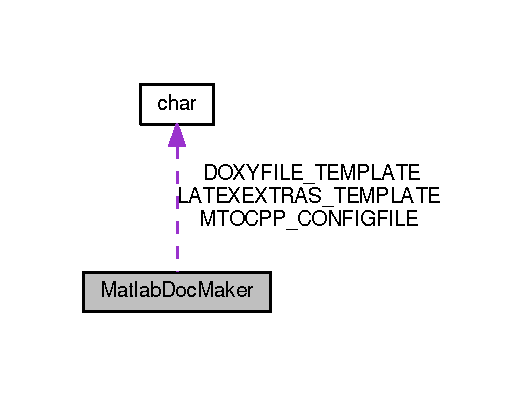
\includegraphics[width=252pt]{class_matlab_doc_maker__coll__graph}
\end{center}
\end{figure}
\subsubsection*{Static Public Member Functions}
\begin{DoxyCompactItemize}
\item 
static mlhs\+Inner\+Subst$<$\+::\hyperlink{classchar}{char}, name $>$ \hyperlink{class_matlab_doc_maker_a9f84ff8d3f39824b54626862780b342c}{get\+Project\+Name} ()
\begin{DoxyCompactList}\small\item\em Returns the project name. \end{DoxyCompactList}\item 
static mlhs\+Inner\+Subst$<$\+::\hyperlink{classchar}{char}, dir $>$ \hyperlink{class_matlab_doc_maker_a1957c12ff4fb6a9d8e1b009961a5f499}{get\+Output\+Directory} ()
\begin{DoxyCompactList}\small\item\em Returns the directory where the applications source files reside. \end{DoxyCompactList}\item 
static mlhs\+Inner\+Subst$<$\+::\hyperlink{classchar}{char}, dir $>$ \hyperlink{class_matlab_doc_maker_a1481c6e95be338b758ec97b8090ee7c9}{get\+Source\+Directory} ()
\begin{DoxyCompactList}\small\item\em Returns the directory where the applications source files reside. \end{DoxyCompactList}\item 
static mlhs\+Inner\+Subst$<$\+::\hyperlink{classchar}{char}, dir $>$ \hyperlink{class_matlab_doc_maker_a11a2a8ec616df969a911b325e39b0b4f}{get\+Config\+Directory} ()
\begin{DoxyCompactList}\small\item\em Returns the directory where the applications documentation configuration files reside. \end{DoxyCompactList}\item 
static mlhs\+Inner\+Subst$<$\+::\hyperlink{classchar}{char}, desc $>$ \hyperlink{class_matlab_doc_maker_af63bb7f2a5008a7b786d2b83b4f72b1b}{get\+Project\+Description} ()
\begin{DoxyCompactList}\small\item\em Returns the short project description. \end{DoxyCompactList}\item 
static noret\+::substitute \hyperlink{class_matlab_doc_maker_a88037a33f6ed26b8b3e60e1cbfd5dfd6}{set\+Project\+Description} (\+::\hyperlink{classchar}{char} value)
\begin{DoxyCompactList}\small\item\em Sets the project description. \end{DoxyCompactList}\item 
static mlhs\+Inner\+Subst$<$\+::\hyperlink{classchar}{char}, version $>$ \hyperlink{class_matlab_doc_maker_afce5384fb7c395546431b7a6c4e1f790}{get\+Project\+Version} ()
\begin{DoxyCompactList}\small\item\em Returns the current version of the project. \end{DoxyCompactList}\item 
static noret\+::substitute \hyperlink{class_matlab_doc_maker_a532ff6bc4beaeff5c3d2f12305bbaa5d}{set\+Project\+Version} (\+::\hyperlink{classchar}{char} value)
\begin{DoxyCompactList}\small\item\em Sets the project version. \end{DoxyCompactList}\item 
static mlhs\+Inner\+Subst$<$ matlabtypesubstitute, full\+Path $>$ \hyperlink{class_matlab_doc_maker_a6767085b13dc2600cb6beda7f7d6acd9}{get\+Project\+Logo} ()
\begin{DoxyCompactList}\small\item\em Returns the logo image file for the project. Either an absolute path or a plain filename. For the latter case the image file is assumed to reside inside the directory returned by \hyperlink{class_matlab_doc_maker_a11a2a8ec616df969a911b325e39b0b4f}{Matlab\+Doc\+Maker.\+get\+Config\+Directory}. \end{DoxyCompactList}\item 
static noret\+::substitute \hyperlink{class_matlab_doc_maker_a6e84afe2189a851665133b6e7c412d4c}{set\+Project\+Logo} (\+::\hyperlink{classchar}{char} value)
\begin{DoxyCompactList}\small\item\em Sets the project logo. Set to \textquotesingle{} to unset. \end{DoxyCompactList}\item 
static noret\+::substitute \hyperlink{class_matlab_doc_maker_ac0a03050ca09039ccd6a1fc97367a38b}{open} ()
\begin{DoxyCompactList}\small\item\em Opens the generated documentation. \end{DoxyCompactList}\item 
static noret\+::substitute \hyperlink{class_matlab_doc_maker_a278883e6b83f6c6e7780e0d567dee119}{create} (matlabtypesubstitute \hyperlink{classvarargin}{varargin})
\begin{DoxyCompactList}\small\item\em Creates the Doxygen documentation. \end{DoxyCompactList}\item 
static noret\+::substitute \hyperlink{class_matlab_doc_maker_a434c176c2421dd18a40003919b19f4f2}{setup} ()
\begin{DoxyCompactList}\small\item\em Runs the setup script for \hyperlink{class_matlab_doc_maker}{Matlab\+Doc\+Maker} and collects all necessary paths in order for the documentation creation to work properly. \end{DoxyCompactList}\end{DoxyCompactItemize}
\subsubsection*{Static Public Attributes}
\begin{DoxyCompactItemize}
\item 
static const \+::\hyperlink{classchar}{char} \hyperlink{class_matlab_doc_maker_ab9514d0ba074c3b92a7fae2b50846b90}{D\+O\+X\+Y\+F\+I\+L\+E\+\_\+\+T\+E\+M\+P\+L\+A\+TE} = \char`\"{}Doxyfile.\+template\char`\"{}
\begin{DoxyCompactList}\small\item\em File name for the doxygen configuration file processed by the \hyperlink{class_matlab_doc_maker}{Matlab\+Doc\+Maker}. \end{DoxyCompactList}\item 
static const \+::\hyperlink{classchar}{char} \hyperlink{class_matlab_doc_maker_a5fd9647b943b91d54acbfce17d0d7416}{L\+A\+T\+E\+X\+E\+X\+T\+R\+A\+S\+\_\+\+T\+E\+M\+P\+L\+A\+TE} = \char`\"{}latexextras.\+template\char`\"{}
\begin{DoxyCompactList}\small\item\em File name for the latex extras style file processed by the \hyperlink{class_matlab_doc_maker}{Matlab\+Doc\+Maker}. \end{DoxyCompactList}\item 
static const \+::\hyperlink{classchar}{char} \hyperlink{class_matlab_doc_maker_ab61ab79ccd92642c4fef74c6abbee559}{M\+T\+O\+C\+P\+P\+\_\+\+C\+O\+N\+F\+I\+G\+F\+I\+LE} = \char`\"{}mtocpp.\+conf\char`\"{}
\begin{DoxyCompactList}\small\item\em File name the mtoc++ configuration file. \end{DoxyCompactList}\end{DoxyCompactItemize}


\subsubsection{Detailed Description}
\hyperlink{class_matlab_doc_maker}{Matlab\+Doc\+Maker}\+: Automated documentation creation using doxygen and mtoc++ from within Mat\+Lab. 

Currently documentation creation for unix and windows environment is supported.

\begin{DoxyParagraph}{Prerequisites}
The following tools must be installed and present on the P\+A\+TH or reside inside the folder returned by \hyperlink{class_matlab_doc_maker_a11a2a8ec616df969a911b325e39b0b4f}{Matlab\+Doc\+Maker.\+get\+Config\+Directory}.
\begin{DoxyItemize}
\item {\ttfamily mtocpp}, {\ttfamily mtocpp\+\_\+post} (the main tool)
\item {\ttfamily doxygen} (mtoc++ is a filter for doxygen)
\end{DoxyItemize}
\end{DoxyParagraph}
\begin{DoxyParagraph}{Strongly recommended}

\begin{DoxyItemize}
\item {\ttfamily latex} Doxygen supports built-\/in latex formulas and Matlab\+Doc\+Maker/mtoc++ allows for easy extra latex inclusions and notation in code
\item {\ttfamily dot} Doxygen creates really nice inheritance graphs and collaboration diagrams with dot.
\end{DoxyItemize}
\end{DoxyParagraph}
\begin{DoxyAuthor}{Author}
Daniel Wirtz 
\end{DoxyAuthor}
\begin{DoxyDate}{Date}
2011-\/10-\/13
\end{DoxyDate}
\begin{DoxyRefDesc}{Change in 1.\+5}
\item[\hyperlink{changelog1_5__changelog1_5000001}{Change in 1.\+5}](dw, 2013-\/12-\/03) Fixed default value selection for properties, now not having set a description or logo does not cause an error to be thrown.\end{DoxyRefDesc}


\begin{DoxyRefDesc}{Change in 1.\+5}
\item[\hyperlink{changelog1_5__changelog1_5000002}{Change in 1.\+5}](dw, 2013-\/02-\/21) Fixed the callback for suggested direct documentation creation after \hyperlink{class_matlab_doc_maker_a434c176c2421dd18a40003919b19f4f2}{Matlab\+Doc\+Maker.\+setup} (Thanks to Aurelien Queffurust)\end{DoxyRefDesc}


\begin{DoxyRefDesc}{Change in 1.\+5}
\item[\hyperlink{changelog1_5__changelog1_5000003}{Change in 1.\+5}](dw, 2013-\/02-\/12) Also added the escaping for the Logo file. Thanks to Chris Olien for the hint.\end{DoxyRefDesc}


\begin{DoxyRefDesc}{Change in 1.\+5}
\item[\hyperlink{changelog1_5__changelog1_5000004}{Change in 1.\+5}](dw, 2013-\/01-\/07) Included some backslash escaping for paths on windows platforms. Thanks to Math\+Works Pilot Engineer \textquotesingle{}{\ttfamily Arvind Jayaraman}\textquotesingle{} for providing the feedback and code!\end{DoxyRefDesc}


\begin{DoxyRefDesc}{Change in 1.\+4}
\item[\hyperlink{changelog1_4__changelog1_4000001}{Change in 1.\+4}](dw, 2012-\/10-\/18) Removed {\ttfamily m4} dependency and included constant properties for configuration file names.\end{DoxyRefDesc}


\begin{DoxyRefDesc}{New in 1.\+4}
\item[\hyperlink{newfeat1_4__newfeat1_4000001}{New in 1.\+4}](dw, 2012-\/10-\/16)
\begin{DoxyItemize}
\item Added two more configuration variables \char`\"{}\+Project\+Description\char`\"{} and \char`\"{}\+Project\+Logo\char`\"{} for easier configuration of the \hyperlink{class_matlab_doc_maker}{Matlab\+Doc\+Maker} in many cases. Thanks to Wolfgang Mennerich \href{http://www.mathworks.com/matlabcentral/fileexchange/authors/272859}{\tt http\+://www.\+mathworks.\+com/matlabcentral/fileexchange/authors/272859} for the suggestion.
\item Restructured the configuration, now only the project name function has to be implemented (the preferences tag depends on it, there might be more than one project within the same Matlab installation whos documentation is created using this tool). The rest can be provided either at setup time or later via suitable setters for the version, description and logo.
\item Automatically setting Have\+Dot in the doxygen config whenever its found on the environment path.
\item Added basic support for La\+TeX documentation creation. Using the parameter {\ttfamily latex}=true for the create method creates the La\+TeX version of the documentation in a folder \char`\"{}latex\char`\"{} in the Output\+Directory (default behaviour)
\end{DoxyItemize}\end{DoxyRefDesc}


\begin{DoxyRefDesc}{Change in 1.\+4}
\item[\hyperlink{changelog1_4__changelog1_4000002}{Change in 1.\+4}](dw, 2012-\/09-\/27) Added automatic dot Graphviz tool detection on call to create.\end{DoxyRefDesc}


\begin{DoxyRefDesc}{Change in 1.\+3}
\item[\hyperlink{changelog1_3__changelog1_3000001}{Change in 1.\+3}](dw, 2012-\/02-\/16)
\begin{DoxyItemize}
\item Now also collecting error messages from mtocpp\+\_\+post and adding them to the warnings.\+log file.
\item Added the directive \char`\"{}\+L\+D\+\_\+\+L\+I\+B\+R\+A\+R\+Y\+\_\+\+P\+A\+T\+H= \char`\"{} for unix systems, as Mat\+Lab sets it inside its executing environment. This can lead to errors if doxygen and/or mtoc++ have been built using never G\+L\+I\+BC (libstd) versions than the one shipped with Mat\+Lab.
\end{DoxyItemize}\end{DoxyRefDesc}


\begin{DoxyRefDesc}{Change in 1.\+3}
\item[\hyperlink{changelog1_3__changelog1_3000002}{Change in 1.\+3}](dw, 2012-\/01-\/16)
\begin{DoxyItemize}
\item Properly using the correct file separators everywhere now
\item Hyperlinked the log file so it can be opened directly
\end{DoxyItemize}\end{DoxyRefDesc}


\begin{DoxyRefDesc}{Change in 1.\+3}
\item[\hyperlink{changelog1_3__changelog1_3000003}{Change in 1.\+3}](dw, 2012-\/01-\/14) Not displaying the \char`\"{}generated warnings\char`\"{}-\/text if there have not been any during documentation creation.\end{DoxyRefDesc}


\begin{DoxyRefDesc}{Change in 1.\+2}
\item[\hyperlink{changelog1_2__changelog1_2000001}{Change in 1.\+2}](dw, 2011-\/11-\/27)
\begin{DoxyItemize}
\item Included documentation creation for the Windows platform and combined the old methods into one (small effective differences)
\item No longer storing the doxygen binary file in the prefs as a lot of tools must be present on the path anyways. The new paradigm is to expect all required 3rd-\/party programmes to be available on P\+A\+TH. As backup the configuration files directory is added to the Matlab P\+A\+TH environment {\bfseries nonpermanently} and any executables found there will thus also be usable.
\item Included checks for {\ttfamily dot} and {\ttfamily latex} at the setup stage to recommend installation of those tools if not present (the default doxygen settings in Doxyfile.\+m4 are to use both)
\end{DoxyItemize}\end{DoxyRefDesc}


\begin{DoxyRefDesc}{Change in 1.\+2}
\item[\hyperlink{changelog1_2__changelog1_2000002}{Change in 1.\+2}](dw, 2011-\/11-\/08) Improved the create\+Unix method by displaying the warnings and writing the output to a log file afterwards. Not using cprintf anymore as this is 3rd party software.\end{DoxyRefDesc}


\begin{DoxyRefDesc}{Change in 1.\+2}
\item[\hyperlink{changelog1_2__changelog1_2000003}{Change in 1.\+2}](dw, 2011-\/11-\/07) Fixed a recursion bug caused by copy and paste. Now the preferences are stored on an per-\/application basis.\end{DoxyRefDesc}


\begin{DoxyRefDesc}{Change in 1.\+2}
\item[\hyperlink{changelog1_2__changelog1_2000004}{Change in 1.\+2}](dw, 2011-\/11-\/04) Changed the name to \hyperlink{class_matlab_doc_maker}{Matlab\+Doc\+Maker} in order to export it into the mtoc++ distribution later.\end{DoxyRefDesc}


\begin{DoxyRefDesc}{New in 1.\+2}
\item[\hyperlink{newfeat1_2__newfeat1_2000001}{New in 1.\+2}](dw, 2011-\/10-\/13) Added this class and moved documentation related stuff here from the Ker\+Mor class.\end{DoxyRefDesc}


This class is part of the mtoc++ tool
\begin{DoxyItemize}
\item {\ttfamily Homepage} \href{http://www.morepas.org/software/mtocpp/}{\tt http\+://www.\+morepas.\+org/software/mtocpp/}
\item {\ttfamily License} \href{http://www.morepas.org/software/mtocpp/docs/licensing.html}{\tt http\+://www.\+morepas.\+org/software/mtocpp/docs/licensing.\+html}
\end{DoxyItemize}

Copyright (c) 2012, Daniel Wirtz All rights reserved.

Redistribution and use in source and binary forms, with or without modification, are permitted only in compliance with the B\+SD license, see \href{http://www.opensource.org/licenses/bsd-license.php}{\tt http\+://www.\+opensource.\+org/licenses/bsd-\/license.\+php} 

Definition at line 17 of file Matlab\+Doc\+Maker.\+m.



\subsubsection{Member Function Documentation}
\index{Matlab\+Doc\+Maker@{Matlab\+Doc\+Maker}!create@{create}}
\index{create@{create}!Matlab\+Doc\+Maker@{Matlab\+Doc\+Maker}}
\paragraph[{\texorpdfstring{create(matlabtypesubstitute varargin)}{create(matlabtypesubstitute varargin)}}]{\setlength{\rightskip}{0pt plus 5cm}noret\+::substitute Matlab\+Doc\+Maker\+::create (
\begin{DoxyParamCaption}
\item[{matlabtypesubstitute}]{varargin}
\end{DoxyParamCaption}
)\hspace{0.3cm}{\ttfamily [static]}}\hypertarget{class_matlab_doc_maker_a278883e6b83f6c6e7780e0d567dee119}{}\label{class_matlab_doc_maker_a278883e6b83f6c6e7780e0d567dee119}


Creates the Doxygen documentation. 


\begin{DoxyParams}{Parameters}
{\em varargin} & Optional parameters for creation. 
\begin{DoxyCode}
\hyperlink{class_matlab_doc_maker_a278883e6b83f6c6e7780e0d567dee119}{create} (  [ \textcolor{stringliteral}{"open"}, open\_value ] [, \textcolor{stringliteral}{"latex"}, latex\_value ] ) 
\end{DoxyCode}
 {\itshape Named Parameters for varargin\+:}
\begin{DoxyItemize}
\item  open Set to true if the documentation should be opened after successful compilation {\bfseries Default\+:} false
\item  latex Set to true if $\text{\LaTeX}$ output should be generated, too. {\bfseries Default\+:} false
\end{DoxyItemize}\\
\hline
\end{DoxyParams}


Definition at line 412 of file Matlab\+Doc\+Maker.\+m.



References D\+O\+X\+Y\+F\+I\+L\+E\+\_\+\+T\+E\+M\+P\+L\+A\+TE, get\+Config\+Directory(), get\+Output\+Directory(), get\+Project\+Description(), get\+Project\+Logo(), get\+Project\+Name(), get\+Project\+Version(), get\+Source\+Directory(), L\+A\+T\+E\+X\+E\+X\+T\+R\+A\+S\+\_\+\+T\+E\+M\+P\+L\+A\+TE, M\+T\+O\+C\+P\+P\+\_\+\+C\+O\+N\+F\+I\+G\+F\+I\+LE, and open().

Here is the call graph for this function\+:
\nopagebreak
\begin{figure}[H]
\begin{center}
\leavevmode
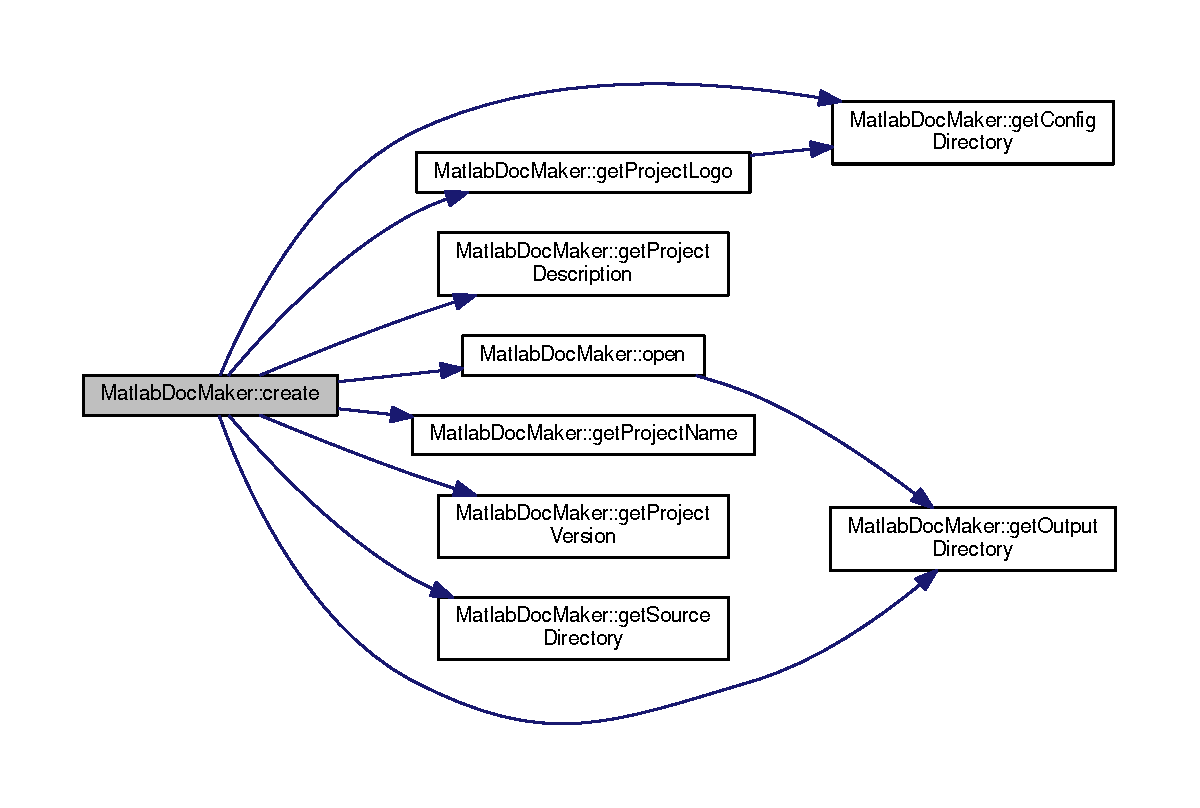
\includegraphics[width=350pt]{class_matlab_doc_maker_a278883e6b83f6c6e7780e0d567dee119_cgraph}
\end{center}
\end{figure}
\index{Matlab\+Doc\+Maker@{Matlab\+Doc\+Maker}!get\+Config\+Directory@{get\+Config\+Directory}}
\index{get\+Config\+Directory@{get\+Config\+Directory}!Matlab\+Doc\+Maker@{Matlab\+Doc\+Maker}}
\paragraph[{\texorpdfstring{get\+Config\+Directory()}{getConfigDirectory()}}]{\setlength{\rightskip}{0pt plus 5cm}mlhs\+Inner\+Subst$<$\+::{\bf char}, dir $>$ Matlab\+Doc\+Maker\+::get\+Config\+Directory (
\begin{DoxyParamCaption}
{}
\end{DoxyParamCaption}
)\hspace{0.3cm}{\ttfamily [static]}}\hypertarget{class_matlab_doc_maker_a11a2a8ec616df969a911b325e39b0b4f}{}\label{class_matlab_doc_maker_a11a2a8ec616df969a911b325e39b0b4f}


Returns the directory where the applications documentation configuration files reside. 

This folder must contain at least the files \char`\"{}mtoc.\+conf\char`\"{} and \char`\"{}\+Doxyfile.\+template\char`\"{}


\begin{DoxyRetVals}{Return values}
{\em dir} & The documentation configuration directory\\
\hline
\end{DoxyRetVals}
\begin{DoxyNote}{Note}
This method has the M\+A\+T\+L\+AB method attribute {\ttfamily Sealed} set to true. It cannot be overwritten. 

\href{http://www.mathworks.com/help/matlab/matlab_oop/method-attributes.html}{\tt matlab documentation of method attributes.} 
\end{DoxyNote}


Definition at line 225 of file Matlab\+Doc\+Maker.\+m.



Referenced by create(), get\+Project\+Logo(), and set\+Project\+Logo().

Here is the caller graph for this function\+:
\nopagebreak
\begin{figure}[H]
\begin{center}
\leavevmode
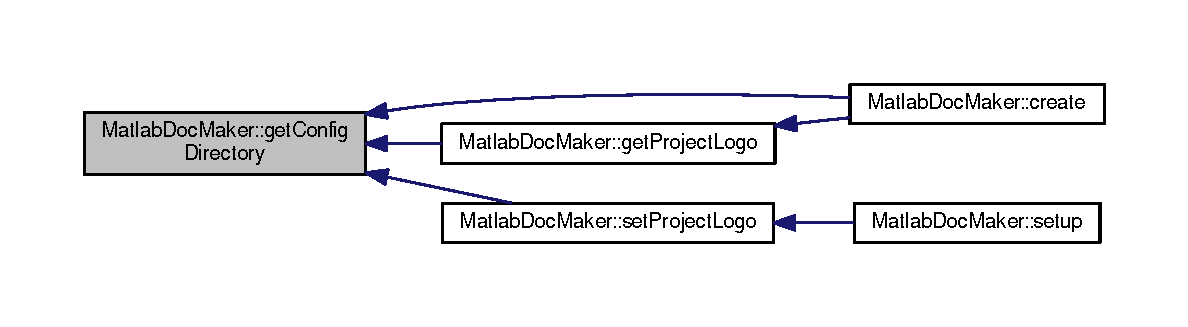
\includegraphics[width=350pt]{class_matlab_doc_maker_a11a2a8ec616df969a911b325e39b0b4f_icgraph}
\end{center}
\end{figure}
\index{Matlab\+Doc\+Maker@{Matlab\+Doc\+Maker}!get\+Output\+Directory@{get\+Output\+Directory}}
\index{get\+Output\+Directory@{get\+Output\+Directory}!Matlab\+Doc\+Maker@{Matlab\+Doc\+Maker}}
\paragraph[{\texorpdfstring{get\+Output\+Directory()}{getOutputDirectory()}}]{\setlength{\rightskip}{0pt plus 5cm}mlhs\+Inner\+Subst$<$\+::{\bf char}, dir $>$ Matlab\+Doc\+Maker\+::get\+Output\+Directory (
\begin{DoxyParamCaption}
{}
\end{DoxyParamCaption}
)\hspace{0.3cm}{\ttfamily [static]}}\hypertarget{class_matlab_doc_maker_a1957c12ff4fb6a9d8e1b009961a5f499}{}\label{class_matlab_doc_maker_a1957c12ff4fb6a9d8e1b009961a5f499}


Returns the directory where the applications source files reside. 


\begin{DoxyRetVals}{Return values}
{\em dir} & The output directory\\
\hline
\end{DoxyRetVals}
\begin{DoxyNote}{Note}
This method has the M\+A\+T\+L\+AB method attribute {\ttfamily Sealed} set to true. It cannot be overwritten. 

\href{http://www.mathworks.com/help/matlab/matlab_oop/method-attributes.html}{\tt matlab documentation of method attributes.} 
\end{DoxyNote}


Definition at line 195 of file Matlab\+Doc\+Maker.\+m.



Referenced by create(), and open().

Here is the caller graph for this function\+:
\nopagebreak
\begin{figure}[H]
\begin{center}
\leavevmode
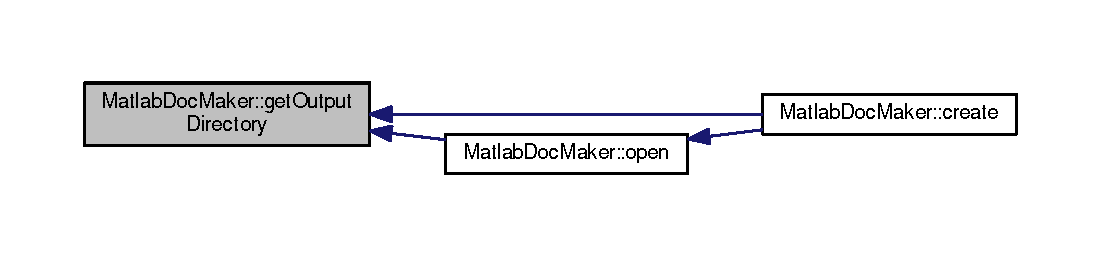
\includegraphics[width=350pt]{class_matlab_doc_maker_a1957c12ff4fb6a9d8e1b009961a5f499_icgraph}
\end{center}
\end{figure}
\index{Matlab\+Doc\+Maker@{Matlab\+Doc\+Maker}!get\+Project\+Description@{get\+Project\+Description}}
\index{get\+Project\+Description@{get\+Project\+Description}!Matlab\+Doc\+Maker@{Matlab\+Doc\+Maker}}
\paragraph[{\texorpdfstring{get\+Project\+Description()}{getProjectDescription()}}]{\setlength{\rightskip}{0pt plus 5cm}mlhs\+Inner\+Subst$<$\+::{\bf char}, desc $>$ Matlab\+Doc\+Maker\+::get\+Project\+Description (
\begin{DoxyParamCaption}
{}
\end{DoxyParamCaption}
)\hspace{0.3cm}{\ttfamily [static]}}\hypertarget{class_matlab_doc_maker_af63bb7f2a5008a7b786d2b83b4f72b1b}{}\label{class_matlab_doc_maker_af63bb7f2a5008a7b786d2b83b4f72b1b}


Returns the short project description. 

\begin{DoxySeeAlso}{See also}
\hyperlink{class_matlab_doc_maker_a88037a33f6ed26b8b3e60e1cbfd5dfd6}{set\+Project\+Description}
\end{DoxySeeAlso}

\begin{DoxyRetVals}{Return values}
{\em desc} & The short project description \\
\hline
\end{DoxyRetVals}
\begin{DoxyParagraph}{Default\+:}
\mbox{[}\mbox{]}
\end{DoxyParagraph}
\begin{DoxyNote}{Note}
This method has the M\+A\+T\+L\+AB method attribute {\ttfamily Sealed} set to true. It cannot be overwritten. 

\href{http://www.mathworks.com/help/matlab/matlab_oop/method-attributes.html}{\tt matlab documentation of method attributes.} 
\end{DoxyNote}


Definition at line 244 of file Matlab\+Doc\+Maker.\+m.



Referenced by create().

Here is the caller graph for this function\+:
\nopagebreak
\begin{figure}[H]
\begin{center}
\leavevmode
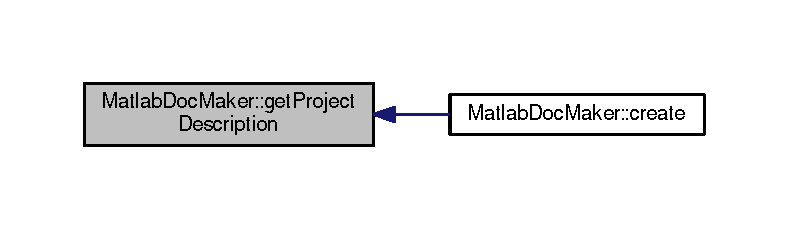
\includegraphics[width=350pt]{class_matlab_doc_maker_af63bb7f2a5008a7b786d2b83b4f72b1b_icgraph}
\end{center}
\end{figure}
\index{Matlab\+Doc\+Maker@{Matlab\+Doc\+Maker}!get\+Project\+Logo@{get\+Project\+Logo}}
\index{get\+Project\+Logo@{get\+Project\+Logo}!Matlab\+Doc\+Maker@{Matlab\+Doc\+Maker}}
\paragraph[{\texorpdfstring{get\+Project\+Logo()}{getProjectLogo()}}]{\setlength{\rightskip}{0pt plus 5cm}mlhs\+Inner\+Subst$<$ matlabtypesubstitute, full\+Path $>$ Matlab\+Doc\+Maker\+::get\+Project\+Logo (
\begin{DoxyParamCaption}
{}
\end{DoxyParamCaption}
)\hspace{0.3cm}{\ttfamily [static]}}\hypertarget{class_matlab_doc_maker_a6767085b13dc2600cb6beda7f7d6acd9}{}\label{class_matlab_doc_maker_a6767085b13dc2600cb6beda7f7d6acd9}


Returns the logo image file for the project. Either an absolute path or a plain filename. For the latter case the image file is assumed to reside inside the directory returned by \hyperlink{class_matlab_doc_maker_a11a2a8ec616df969a911b325e39b0b4f}{Matlab\+Doc\+Maker.\+get\+Config\+Directory}. 

\begin{DoxySeeAlso}{See also}
\hyperlink{class_matlab_doc_maker_a6e84afe2189a851665133b6e7c412d4c}{set\+Project\+Logo}
\end{DoxySeeAlso}

\begin{DoxyRetVals}{Return values}
{\em logo\+File} & The projects logo image file. \\
\hline
\end{DoxyRetVals}
\begin{DoxyParagraph}{Default\+:}
\mbox{[}\mbox{]}
\end{DoxyParagraph}
\begin{DoxyNote}{Note}
This method has the M\+A\+T\+L\+AB method attribute {\ttfamily Sealed} set to true. It cannot be overwritten. 

\href{http://www.mathworks.com/help/matlab/matlab_oop/method-attributes.html}{\tt matlab documentation of method attributes.} 
\end{DoxyNote}


Definition at line 317 of file Matlab\+Doc\+Maker.\+m.



References get\+Config\+Directory().



Referenced by create().

Here is the call graph for this function\+:
\nopagebreak
\begin{figure}[H]
\begin{center}
\leavevmode
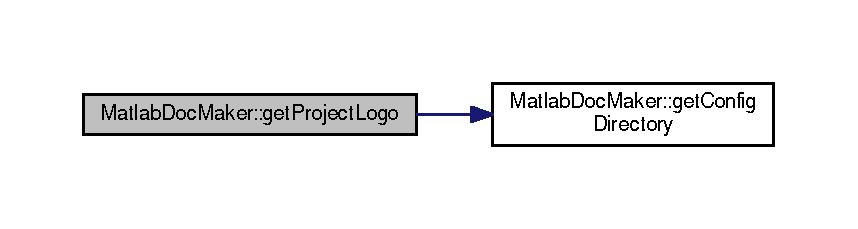
\includegraphics[width=350pt]{class_matlab_doc_maker_a6767085b13dc2600cb6beda7f7d6acd9_cgraph}
\end{center}
\end{figure}
Here is the caller graph for this function\+:
\nopagebreak
\begin{figure}[H]
\begin{center}
\leavevmode
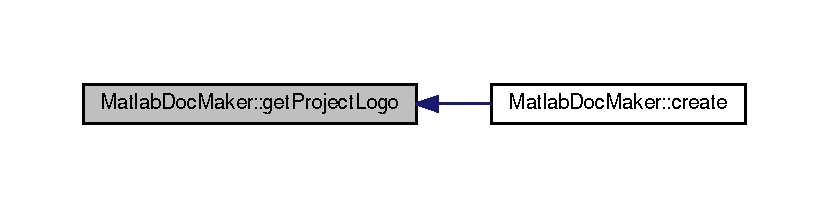
\includegraphics[width=350pt]{class_matlab_doc_maker_a6767085b13dc2600cb6beda7f7d6acd9_icgraph}
\end{center}
\end{figure}
\index{Matlab\+Doc\+Maker@{Matlab\+Doc\+Maker}!get\+Project\+Name@{get\+Project\+Name}}
\index{get\+Project\+Name@{get\+Project\+Name}!Matlab\+Doc\+Maker@{Matlab\+Doc\+Maker}}
\paragraph[{\texorpdfstring{get\+Project\+Name()}{getProjectName()}}]{\setlength{\rightskip}{0pt plus 5cm}mlhs\+Inner\+Subst$<$\+::{\bf char}, name $>$ Matlab\+Doc\+Maker\+::get\+Project\+Name (
\begin{DoxyParamCaption}
{}
\end{DoxyParamCaption}
)\hspace{0.3cm}{\ttfamily [static]}}\hypertarget{class_matlab_doc_maker_a9f84ff8d3f39824b54626862780b342c}{}\label{class_matlab_doc_maker_a9f84ff8d3f39824b54626862780b342c}


Returns the project name. 

\begin{DoxyNote}{Note}
Changing the return value of this method will require another execution of \hyperlink{class_matlab_doc_maker_a434c176c2421dd18a40003919b19f4f2}{Matlab\+Doc\+Maker.\+setup} as the preferences storage key also depends on it.
\end{DoxyNote}

\begin{DoxyRetVals}{Return values}
{\em name} & The project name \\
\hline
\end{DoxyRetVals}


Definition at line 170 of file Matlab\+Doc\+Maker.\+m.



Referenced by create(), and setup().

Here is the caller graph for this function\+:
\nopagebreak
\begin{figure}[H]
\begin{center}
\leavevmode
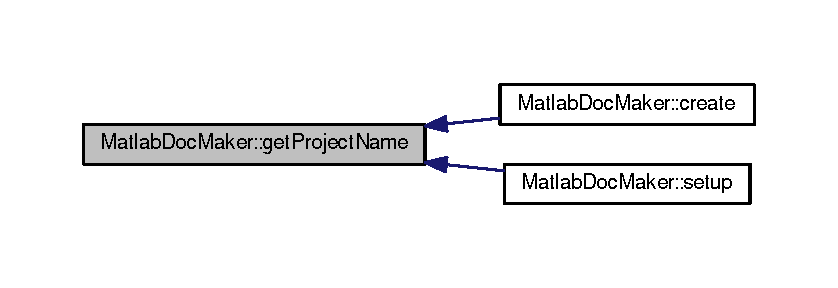
\includegraphics[width=350pt]{class_matlab_doc_maker_a9f84ff8d3f39824b54626862780b342c_icgraph}
\end{center}
\end{figure}
\index{Matlab\+Doc\+Maker@{Matlab\+Doc\+Maker}!get\+Project\+Version@{get\+Project\+Version}}
\index{get\+Project\+Version@{get\+Project\+Version}!Matlab\+Doc\+Maker@{Matlab\+Doc\+Maker}}
\paragraph[{\texorpdfstring{get\+Project\+Version()}{getProjectVersion()}}]{\setlength{\rightskip}{0pt plus 5cm}mlhs\+Inner\+Subst$<$\+::{\bf char}, version $>$ Matlab\+Doc\+Maker\+::get\+Project\+Version (
\begin{DoxyParamCaption}
{}
\end{DoxyParamCaption}
)\hspace{0.3cm}{\ttfamily [static]}}\hypertarget{class_matlab_doc_maker_afce5384fb7c395546431b7a6c4e1f790}{}\label{class_matlab_doc_maker_afce5384fb7c395546431b7a6c4e1f790}


Returns the current version of the project. 

\begin{DoxyNote}{Note}
The built-\/in @new and @change tags from the Doxyfile.\+template support two-\/level versioning a la X.\+X.
\end{DoxyNote}
\begin{DoxySeeAlso}{See also}
\hyperlink{class_matlab_doc_maker_a532ff6bc4beaeff5c3d2f12305bbaa5d}{set\+Project\+Version}
\end{DoxySeeAlso}

\begin{DoxyRetVals}{Return values}
{\em version} & The project version \\
\hline
\end{DoxyRetVals}
\begin{DoxyParagraph}{Default\+:}
\mbox{[}\mbox{]}
\end{DoxyParagraph}
\begin{DoxyNote}{Note}
This method has the M\+A\+T\+L\+AB method attribute {\ttfamily Sealed} set to true. It cannot be overwritten. 

\href{http://www.mathworks.com/help/matlab/matlab_oop/method-attributes.html}{\tt matlab documentation of method attributes.} 
\end{DoxyNote}


Definition at line 279 of file Matlab\+Doc\+Maker.\+m.



Referenced by create().

Here is the caller graph for this function\+:
\nopagebreak
\begin{figure}[H]
\begin{center}
\leavevmode
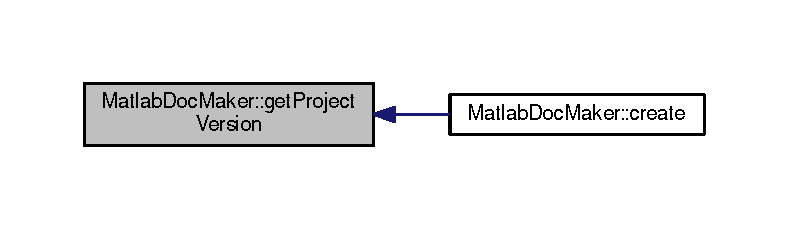
\includegraphics[width=350pt]{class_matlab_doc_maker_afce5384fb7c395546431b7a6c4e1f790_icgraph}
\end{center}
\end{figure}
\index{Matlab\+Doc\+Maker@{Matlab\+Doc\+Maker}!get\+Source\+Directory@{get\+Source\+Directory}}
\index{get\+Source\+Directory@{get\+Source\+Directory}!Matlab\+Doc\+Maker@{Matlab\+Doc\+Maker}}
\paragraph[{\texorpdfstring{get\+Source\+Directory()}{getSourceDirectory()}}]{\setlength{\rightskip}{0pt plus 5cm}mlhs\+Inner\+Subst$<$\+::{\bf char}, dir $>$ Matlab\+Doc\+Maker\+::get\+Source\+Directory (
\begin{DoxyParamCaption}
{}
\end{DoxyParamCaption}
)\hspace{0.3cm}{\ttfamily [static]}}\hypertarget{class_matlab_doc_maker_a1481c6e95be338b758ec97b8090ee7c9}{}\label{class_matlab_doc_maker_a1481c6e95be338b758ec97b8090ee7c9}


Returns the directory where the applications source files reside. 


\begin{DoxyRetVals}{Return values}
{\em dir} & The project source directory\\
\hline
\end{DoxyRetVals}
\begin{DoxyNote}{Note}
This method has the M\+A\+T\+L\+AB method attribute {\ttfamily Sealed} set to true. It cannot be overwritten. 

\href{http://www.mathworks.com/help/matlab/matlab_oop/method-attributes.html}{\tt matlab documentation of method attributes.} 
\end{DoxyNote}


Definition at line 210 of file Matlab\+Doc\+Maker.\+m.



Referenced by create().

Here is the caller graph for this function\+:
\nopagebreak
\begin{figure}[H]
\begin{center}
\leavevmode
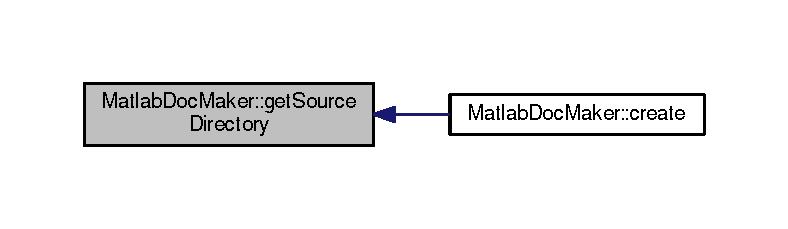
\includegraphics[width=350pt]{class_matlab_doc_maker_a1481c6e95be338b758ec97b8090ee7c9_icgraph}
\end{center}
\end{figure}
\index{Matlab\+Doc\+Maker@{Matlab\+Doc\+Maker}!open@{open}}
\index{open@{open}!Matlab\+Doc\+Maker@{Matlab\+Doc\+Maker}}
\paragraph[{\texorpdfstring{open()}{open()}}]{\setlength{\rightskip}{0pt plus 5cm}noret\+::substitute Matlab\+Doc\+Maker\+::open (
\begin{DoxyParamCaption}
{}
\end{DoxyParamCaption}
)\hspace{0.3cm}{\ttfamily [static]}}\hypertarget{class_matlab_doc_maker_ac0a03050ca09039ccd6a1fc97367a38b}{}\label{class_matlab_doc_maker_ac0a03050ca09039ccd6a1fc97367a38b}


Opens the generated documentation. 

Depending on the system{\ttfamily s type the generated index.\+html is opened in the system}s default browser. 

Definition at line 391 of file Matlab\+Doc\+Maker.\+m.



References get\+Output\+Directory().



Referenced by create().

Here is the call graph for this function\+:
\nopagebreak
\begin{figure}[H]
\begin{center}
\leavevmode
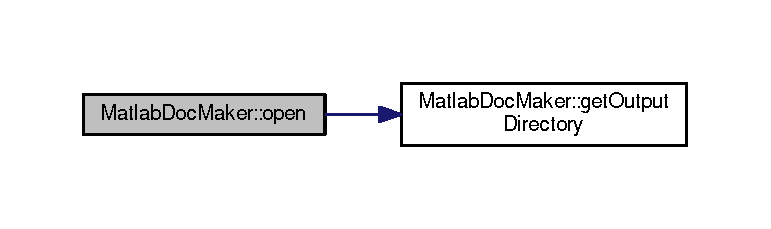
\includegraphics[width=350pt]{class_matlab_doc_maker_ac0a03050ca09039ccd6a1fc97367a38b_cgraph}
\end{center}
\end{figure}
Here is the caller graph for this function\+:
\nopagebreak
\begin{figure}[H]
\begin{center}
\leavevmode
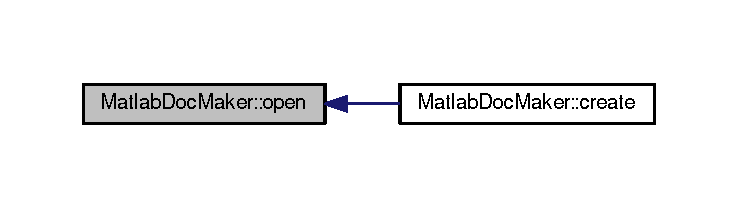
\includegraphics[width=350pt]{class_matlab_doc_maker_ac0a03050ca09039ccd6a1fc97367a38b_icgraph}
\end{center}
\end{figure}
\index{Matlab\+Doc\+Maker@{Matlab\+Doc\+Maker}!set\+Project\+Description@{set\+Project\+Description}}
\index{set\+Project\+Description@{set\+Project\+Description}!Matlab\+Doc\+Maker@{Matlab\+Doc\+Maker}}
\paragraph[{\texorpdfstring{set\+Project\+Description(\+::char value)}{setProjectDescription(::char value)}}]{\setlength{\rightskip}{0pt plus 5cm}noret\+::substitute Matlab\+Doc\+Maker\+::set\+Project\+Description (
\begin{DoxyParamCaption}
\item[{\+::{\bf char}}]{value}
\end{DoxyParamCaption}
)\hspace{0.3cm}{\ttfamily [static]}}\hypertarget{class_matlab_doc_maker_a88037a33f6ed26b8b3e60e1cbfd5dfd6}{}\label{class_matlab_doc_maker_a88037a33f6ed26b8b3e60e1cbfd5dfd6}


Sets the project description. 

\begin{DoxySeeAlso}{See also}
\hyperlink{class_matlab_doc_maker_af63bb7f2a5008a7b786d2b83b4f72b1b}{get\+Project\+Description}
\end{DoxySeeAlso}

\begin{DoxyParams}{Parameters}
{\em value} & The description\\
\hline
\end{DoxyParams}
\begin{DoxyNote}{Note}
This method has the M\+A\+T\+L\+AB method attribute {\ttfamily Sealed} set to true. It cannot be overwritten. 

\href{http://www.mathworks.com/help/matlab/matlab_oop/method-attributes.html}{\tt matlab documentation of method attributes.} 
\end{DoxyNote}


Definition at line 260 of file Matlab\+Doc\+Maker.\+m.

\index{Matlab\+Doc\+Maker@{Matlab\+Doc\+Maker}!set\+Project\+Logo@{set\+Project\+Logo}}
\index{set\+Project\+Logo@{set\+Project\+Logo}!Matlab\+Doc\+Maker@{Matlab\+Doc\+Maker}}
\paragraph[{\texorpdfstring{set\+Project\+Logo(\+::char value)}{setProjectLogo(::char value)}}]{\setlength{\rightskip}{0pt plus 5cm}noret\+::substitute Matlab\+Doc\+Maker\+::set\+Project\+Logo (
\begin{DoxyParamCaption}
\item[{\+::{\bf char}}]{value}
\end{DoxyParamCaption}
)\hspace{0.3cm}{\ttfamily [static]}}\hypertarget{class_matlab_doc_maker_a6e84afe2189a851665133b6e7c412d4c}{}\label{class_matlab_doc_maker_a6e84afe2189a851665133b6e7c412d4c}


Sets the project logo. Set to \textquotesingle{} to unset. 

See the doxygen documentation for valid logo file types (wont be checked here).

\begin{DoxySeeAlso}{See also}
\hyperlink{class_matlab_doc_maker_a6767085b13dc2600cb6beda7f7d6acd9}{get\+Project\+Logo}
\end{DoxySeeAlso}

\begin{DoxyParams}{Parameters}
{\em value} & The logo file to use. Must be either an absolute path or a plain filename, in which case the image is assumed to reside inside the \hyperlink{class_matlab_doc_maker_a11a2a8ec616df969a911b325e39b0b4f}{Matlab\+Doc\+Maker.\+get\+Config\+Directory} directory.\\
\hline
\end{DoxyParams}
\begin{DoxyNote}{Note}
This method has the M\+A\+T\+L\+AB method attribute {\ttfamily Sealed} set to true. It cannot be overwritten. 

\href{http://www.mathworks.com/help/matlab/matlab_oop/method-attributes.html}{\tt matlab documentation of method attributes.} 
\end{DoxyNote}


Definition at line 347 of file Matlab\+Doc\+Maker.\+m.



References get\+Config\+Directory().



Referenced by setup().

Here is the call graph for this function\+:
\nopagebreak
\begin{figure}[H]
\begin{center}
\leavevmode
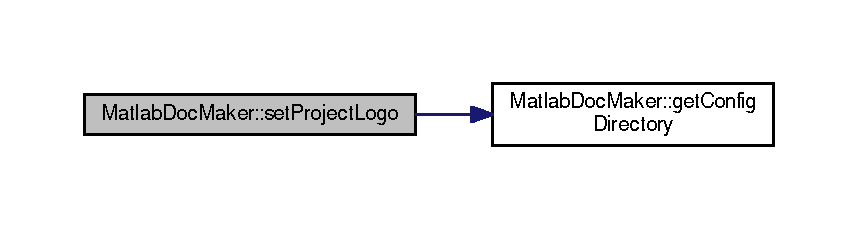
\includegraphics[width=350pt]{class_matlab_doc_maker_a6e84afe2189a851665133b6e7c412d4c_cgraph}
\end{center}
\end{figure}
Here is the caller graph for this function\+:
\nopagebreak
\begin{figure}[H]
\begin{center}
\leavevmode
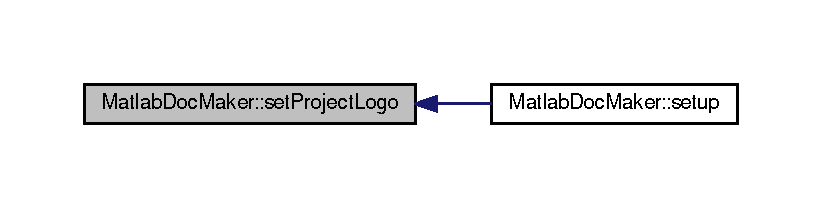
\includegraphics[width=350pt]{class_matlab_doc_maker_a6e84afe2189a851665133b6e7c412d4c_icgraph}
\end{center}
\end{figure}
\index{Matlab\+Doc\+Maker@{Matlab\+Doc\+Maker}!set\+Project\+Version@{set\+Project\+Version}}
\index{set\+Project\+Version@{set\+Project\+Version}!Matlab\+Doc\+Maker@{Matlab\+Doc\+Maker}}
\paragraph[{\texorpdfstring{set\+Project\+Version(\+::char value)}{setProjectVersion(::char value)}}]{\setlength{\rightskip}{0pt plus 5cm}noret\+::substitute Matlab\+Doc\+Maker\+::set\+Project\+Version (
\begin{DoxyParamCaption}
\item[{\+::{\bf char}}]{value}
\end{DoxyParamCaption}
)\hspace{0.3cm}{\ttfamily [static]}}\hypertarget{class_matlab_doc_maker_a532ff6bc4beaeff5c3d2f12305bbaa5d}{}\label{class_matlab_doc_maker_a532ff6bc4beaeff5c3d2f12305bbaa5d}


Sets the project version. 

\begin{DoxySeeAlso}{See also}
\hyperlink{class_matlab_doc_maker_afce5384fb7c395546431b7a6c4e1f790}{get\+Project\+Version}
\end{DoxySeeAlso}

\begin{DoxyParams}{Parameters}
{\em value} & The version string\\
\hline
\end{DoxyParams}
\begin{DoxyNote}{Note}
This method has the M\+A\+T\+L\+AB method attribute {\ttfamily Sealed} set to true. It cannot be overwritten. 

\href{http://www.mathworks.com/help/matlab/matlab_oop/method-attributes.html}{\tt matlab documentation of method attributes.} 
\end{DoxyNote}


Definition at line 298 of file Matlab\+Doc\+Maker.\+m.

\index{Matlab\+Doc\+Maker@{Matlab\+Doc\+Maker}!setup@{setup}}
\index{setup@{setup}!Matlab\+Doc\+Maker@{Matlab\+Doc\+Maker}}
\paragraph[{\texorpdfstring{setup()}{setup()}}]{\setlength{\rightskip}{0pt plus 5cm}noret\+::substitute Matlab\+Doc\+Maker\+::setup (
\begin{DoxyParamCaption}
{}
\end{DoxyParamCaption}
)\hspace{0.3cm}{\ttfamily [static]}}\hypertarget{class_matlab_doc_maker_a434c176c2421dd18a40003919b19f4f2}{}\label{class_matlab_doc_maker_a434c176c2421dd18a40003919b19f4f2}


Runs the setup script for \hyperlink{class_matlab_doc_maker}{Matlab\+Doc\+Maker} and collects all necessary paths in order for the documentation creation to work properly. 



Definition at line 631 of file Matlab\+Doc\+Maker.\+m.



References get\+Project\+Name(), and set\+Project\+Logo().

Here is the call graph for this function\+:
\nopagebreak
\begin{figure}[H]
\begin{center}
\leavevmode
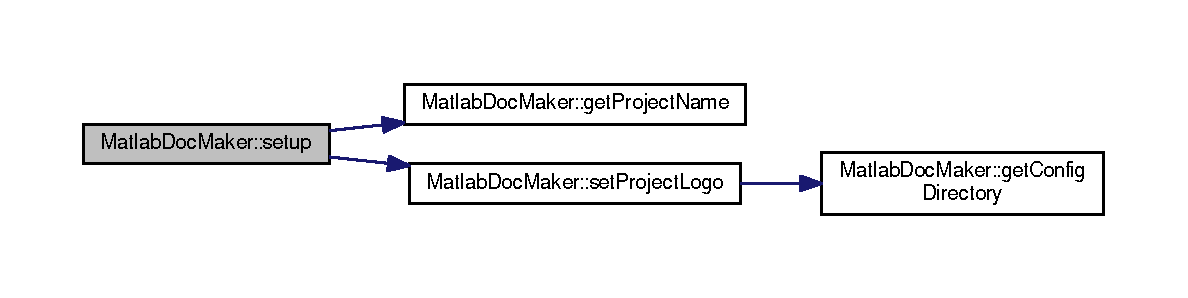
\includegraphics[width=350pt]{class_matlab_doc_maker_a434c176c2421dd18a40003919b19f4f2_cgraph}
\end{center}
\end{figure}


\subsubsection{Member Data Documentation}
\index{Matlab\+Doc\+Maker@{Matlab\+Doc\+Maker}!D\+O\+X\+Y\+F\+I\+L\+E\+\_\+\+T\+E\+M\+P\+L\+A\+TE@{D\+O\+X\+Y\+F\+I\+L\+E\+\_\+\+T\+E\+M\+P\+L\+A\+TE}}
\index{D\+O\+X\+Y\+F\+I\+L\+E\+\_\+\+T\+E\+M\+P\+L\+A\+TE@{D\+O\+X\+Y\+F\+I\+L\+E\+\_\+\+T\+E\+M\+P\+L\+A\+TE}!Matlab\+Doc\+Maker@{Matlab\+Doc\+Maker}}
\paragraph[{\texorpdfstring{D\+O\+X\+Y\+F\+I\+L\+E\+\_\+\+T\+E\+M\+P\+L\+A\+TE}{DOXYFILE\_TEMPLATE}}]{\setlength{\rightskip}{0pt plus 5cm}Matlab\+Doc\+Maker\+::\+D\+O\+X\+Y\+F\+I\+L\+E\+\_\+\+T\+E\+M\+P\+L\+A\+TE = \char`\"{}Doxyfile.\+template\char`\"{}\hspace{0.3cm}{\ttfamily [static]}}\hypertarget{class_matlab_doc_maker_ab9514d0ba074c3b92a7fae2b50846b90}{}\label{class_matlab_doc_maker_ab9514d0ba074c3b92a7fae2b50846b90}


File name for the doxygen configuration file processed by the \hyperlink{class_matlab_doc_maker}{Matlab\+Doc\+Maker}. 

Assumed to reside in the \hyperlink{class_matlab_doc_maker_a11a2a8ec616df969a911b325e39b0b4f}{Matlab\+Doc\+Maker.\+get\+Config\+Directory}

{\bfseries Default\+:} {\ttfamily Doxyfile.\+template} 

Definition at line 130 of file Matlab\+Doc\+Maker.\+m.



Referenced by create().

\index{Matlab\+Doc\+Maker@{Matlab\+Doc\+Maker}!L\+A\+T\+E\+X\+E\+X\+T\+R\+A\+S\+\_\+\+T\+E\+M\+P\+L\+A\+TE@{L\+A\+T\+E\+X\+E\+X\+T\+R\+A\+S\+\_\+\+T\+E\+M\+P\+L\+A\+TE}}
\index{L\+A\+T\+E\+X\+E\+X\+T\+R\+A\+S\+\_\+\+T\+E\+M\+P\+L\+A\+TE@{L\+A\+T\+E\+X\+E\+X\+T\+R\+A\+S\+\_\+\+T\+E\+M\+P\+L\+A\+TE}!Matlab\+Doc\+Maker@{Matlab\+Doc\+Maker}}
\paragraph[{\texorpdfstring{L\+A\+T\+E\+X\+E\+X\+T\+R\+A\+S\+\_\+\+T\+E\+M\+P\+L\+A\+TE}{LATEXEXTRAS\_TEMPLATE}}]{\setlength{\rightskip}{0pt plus 5cm}Matlab\+Doc\+Maker\+::\+L\+A\+T\+E\+X\+E\+X\+T\+R\+A\+S\+\_\+\+T\+E\+M\+P\+L\+A\+TE = \char`\"{}latexextras.\+template\char`\"{}\hspace{0.3cm}{\ttfamily [static]}}\hypertarget{class_matlab_doc_maker_a5fd9647b943b91d54acbfce17d0d7416}{}\label{class_matlab_doc_maker_a5fd9647b943b91d54acbfce17d0d7416}


File name for the latex extras style file processed by the \hyperlink{class_matlab_doc_maker}{Matlab\+Doc\+Maker}. 

Assumed to reside in the \hyperlink{class_matlab_doc_maker_a11a2a8ec616df969a911b325e39b0b4f}{Matlab\+Doc\+Maker.\+get\+Config\+Directory}. If not found, no latex extras are used.

{\bfseries Default\+:} {\ttfamily latexextras.\+template} 

Definition at line 142 of file Matlab\+Doc\+Maker.\+m.



Referenced by create().

\index{Matlab\+Doc\+Maker@{Matlab\+Doc\+Maker}!M\+T\+O\+C\+P\+P\+\_\+\+C\+O\+N\+F\+I\+G\+F\+I\+LE@{M\+T\+O\+C\+P\+P\+\_\+\+C\+O\+N\+F\+I\+G\+F\+I\+LE}}
\index{M\+T\+O\+C\+P\+P\+\_\+\+C\+O\+N\+F\+I\+G\+F\+I\+LE@{M\+T\+O\+C\+P\+P\+\_\+\+C\+O\+N\+F\+I\+G\+F\+I\+LE}!Matlab\+Doc\+Maker@{Matlab\+Doc\+Maker}}
\paragraph[{\texorpdfstring{M\+T\+O\+C\+P\+P\+\_\+\+C\+O\+N\+F\+I\+G\+F\+I\+LE}{MTOCPP\_CONFIGFILE}}]{\setlength{\rightskip}{0pt plus 5cm}Matlab\+Doc\+Maker\+::\+M\+T\+O\+C\+P\+P\+\_\+\+C\+O\+N\+F\+I\+G\+F\+I\+LE = \char`\"{}mtocpp.\+conf\char`\"{}\hspace{0.3cm}{\ttfamily [static]}}\hypertarget{class_matlab_doc_maker_ab61ab79ccd92642c4fef74c6abbee559}{}\label{class_matlab_doc_maker_ab61ab79ccd92642c4fef74c6abbee559}


File name the mtoc++ configuration file. 

Assumed to reside in the \hyperlink{class_matlab_doc_maker_a11a2a8ec616df969a911b325e39b0b4f}{Matlab\+Doc\+Maker.\+get\+Config\+Directory}. If not found, no special configuration is used.

{\bfseries Default\+:} {\ttfamily mtocpp.\+conf} 

Definition at line 155 of file Matlab\+Doc\+Maker.\+m.



Referenced by create().



The documentation for this class was generated from the following file\+:\begin{DoxyCompactItemize}
\item 
\hyperlink{_matlab_doc_maker_8m}{Matlab\+Doc\+Maker.\+m}\end{DoxyCompactItemize}

\hypertarget{classmatrix}{}\subsection{matrix Class Reference}
\label{classmatrix}\index{matrix@{matrix}}


A matlab matrix.  




Inheritance diagram for matrix\+:
\nopagebreak
\begin{figure}[H]
\begin{center}
\leavevmode
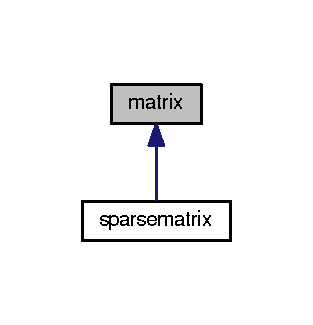
\includegraphics[width=150pt]{classmatrix__inherit__graph}
\end{center}
\end{figure}


\subsubsection{Detailed Description}
A matlab matrix. 

This class is an artificially created class in doxygen to allow more precise type declarations 

Definition at line 73 of file class\+\_\+substitutes.\+c.



The documentation for this class was generated from the following file\+:\begin{DoxyCompactItemize}
\item 
/home/ayonga/\+Dropbox/research/dzopt/direct\+\_\+hzd\+\_\+optimization/docs/config/\hyperlink{class__substitutes_8c}{class\+\_\+substitutes.\+c}\end{DoxyCompactItemize}

\hypertarget{classrowvec}{}\subsection{rowvec Class Reference}
\label{classrowvec}\index{rowvec@{rowvec}}


A matlab row vector.  




\subsubsection{Detailed Description}
A matlab row vector. 

This class is an artificially created class in doxygen to allow more precise type declarations 

The documentation for this class was generated from the following file\+:\begin{DoxyCompactItemize}
\item 
/home/ayonga/\+Dropbox/research/dzopt/direct\+\_\+hzd\+\_\+optimization/docs/config/\hyperlink{class__substitutes_8c}{class\+\_\+substitutes.\+c}\end{DoxyCompactItemize}

\hypertarget{classsparsematrix}{}\subsection{sparsematrix Class Reference}
\label{classsparsematrix}\index{sparsematrix@{sparsematrix}}


A matlab sparse matrix.  




Inheritance diagram for sparsematrix\+:
\nopagebreak
\begin{figure}[H]
\begin{center}
\leavevmode
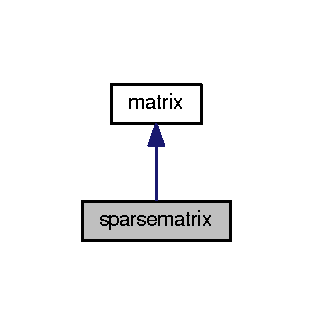
\includegraphics[width=150pt]{classsparsematrix__inherit__graph}
\end{center}
\end{figure}


Collaboration diagram for sparsematrix\+:
\nopagebreak
\begin{figure}[H]
\begin{center}
\leavevmode
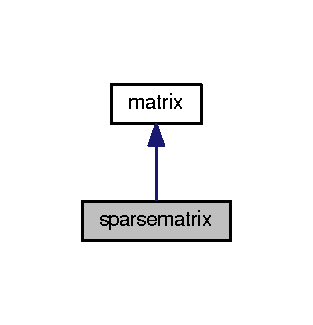
\includegraphics[width=150pt]{classsparsematrix__coll__graph}
\end{center}
\end{figure}


\subsubsection{Detailed Description}
A matlab sparse matrix. 

This class is an artificially created class in doxygen to allow more precise type declarations 

Definition at line 81 of file class\+\_\+substitutes.\+c.



The documentation for this class was generated from the following file\+:\begin{DoxyCompactItemize}
\item 
/home/ayonga/\+Dropbox/research/dzopt/direct\+\_\+hzd\+\_\+optimization/docs/config/\hyperlink{class__substitutes_8c}{class\+\_\+substitutes.\+c}\end{DoxyCompactItemize}

\hypertarget{classstruct}{}\subsection{struct Class Reference}
\label{classstruct}\index{struct@{struct}}


A Mat\+Lab struct.  




\subsubsection{Detailed Description}
A Mat\+Lab struct. 

This class is an artificially created class in doxygen to allow more precise type declarations 

The documentation for this class was generated from the following file\+:\begin{DoxyCompactItemize}
\item 
/home/ayonga/\+Dropbox/research/dzopt/direct\+\_\+hzd\+\_\+optimization/docs/config/\hyperlink{class__substitutes_8c}{class\+\_\+substitutes.\+c}\end{DoxyCompactItemize}

\hypertarget{classvarargin}{}\subsection{varargin Class Reference}
\label{classvarargin}\index{varargin@{varargin}}


A variable number of input arguments.  




\subsubsection{Detailed Description}
A variable number of input arguments. 

This class is an artificially created class in doxygen to allow more precise type declarations.

For more information about the varargin argument see the \href{http://www.mathworks.de/help/techdoc/ref/varargin.html}{\tt Mat\+Lab documentation on varargin}. 

The documentation for this class was generated from the following file\+:\begin{DoxyCompactItemize}
\item 
/home/ayonga/\+Dropbox/research/dzopt/direct\+\_\+hzd\+\_\+optimization/docs/config/\hyperlink{class__substitutes_8c}{class\+\_\+substitutes.\+c}\end{DoxyCompactItemize}

\hypertarget{classvarargout}{}\subsection{varargout Class Reference}
\label{classvarargout}\index{varargout@{varargout}}


A variable number of output arguments.  




\subsubsection{Detailed Description}
A variable number of output arguments. 

This class is an artificially created class in doxygen to allow more precise type declarations.

For more information about the varargout argument see the \href{http://www.mathworks.de/help/techdoc/ref/varargout.html}{\tt Mat\+Lab documentation on varargout}. 

The documentation for this class was generated from the following file\+:\begin{DoxyCompactItemize}
\item 
/home/ayonga/\+Dropbox/research/dzopt/direct\+\_\+hzd\+\_\+optimization/docs/config/\hyperlink{class__substitutes_8c}{class\+\_\+substitutes.\+c}\end{DoxyCompactItemize}

\section{File Documentation}
\hypertarget{class__substitutes_8c}{}\subsection{/home/ayonga/\+Dropbox/research/dzopt/direct\+\_\+hzd\+\_\+optimization/docs/config/class\+\_\+substitutes.c File Reference}
\label{class__substitutes_8c}\index{/home/ayonga/\+Dropbox/research/dzopt/direct\+\_\+hzd\+\_\+optimization/docs/config/class\+\_\+substitutes.\+c@{/home/ayonga/\+Dropbox/research/dzopt/direct\+\_\+hzd\+\_\+optimization/docs/config/class\+\_\+substitutes.\+c}}
\subsubsection*{Classes}
\begin{DoxyCompactItemize}
\item 
class \hyperlink{classmatrix}{matrix}
\begin{DoxyCompactList}\small\item\em A matlab matrix. \end{DoxyCompactList}\item 
class \hyperlink{classsparsematrix}{sparsematrix}
\begin{DoxyCompactList}\small\item\em A matlab sparse matrix. \end{DoxyCompactList}\item 
class \hyperlink{classhandle}{handle}
\begin{DoxyCompactList}\small\item\em Matlab\textquotesingle{}s base handle class (documentation generation substitute) \end{DoxyCompactList}\end{DoxyCompactItemize}

\hypertarget{developers_8c}{}\subsection{/home/ayonga/\+Dropbox/research/dzopt/direct\+\_\+hzd\+\_\+optimization/docs/config/developers.c File Reference}
\label{developers_8c}\index{/home/ayonga/\+Dropbox/research/dzopt/direct\+\_\+hzd\+\_\+optimization/docs/config/developers.\+c@{/home/ayonga/\+Dropbox/research/dzopt/direct\+\_\+hzd\+\_\+optimization/docs/config/developers.\+c}}

\hypertarget{_matlab_doc_maker_8m}{}\subsection{Matlab\+Doc\+Maker.\+m File Reference}
\label{_matlab_doc_maker_8m}\index{Matlab\+Doc\+Maker.\+m@{Matlab\+Doc\+Maker.\+m}}
\subsubsection*{Classes}
\begin{DoxyCompactItemize}
\item 
class \hyperlink{class_matlab_doc_maker}{Matlab\+Doc\+Maker}
\begin{DoxyCompactList}\small\item\em \hyperlink{class_matlab_doc_maker}{Matlab\+Doc\+Maker}\+: Automated documentation creation using doxygen and mtoc++ from within Mat\+Lab. \end{DoxyCompactList}\end{DoxyCompactItemize}

%--- End generated contents ---

% Index
\newpage
\phantomsection
\clearemptydoublepage
\addcontentsline{toc}{section}{Index}
\printindex

\end{document}
